\documentclass[11pt,aspectratio=169]{beamer}
% WiL progress update, 16 November 2026.  Same conventions as update_071126
% and update_221026: one claim per slide, the slide title IS the claim, and
% the data that shows it sits on the same slide.  New in this deck: Part A is
% the methodology -- the visual-SLAM flow as the four reference papers
% describe it, drawn so that every Experiment 1 and 4 finding in Part B can
% point back at the block it lives in.  The slide layout follows the Canva
% deck orb_vins_rtab.pdf in this folder: a numbered section on every slide
% and the paper the slide draws on named in its footer.
\usetheme{default}
\usecolortheme{seagull}
\setbeamertemplate{navigation symbols}{}
\setbeamertemplate{footline}[frame number]
\setbeamerfont{frametitle}{size=\large,series=\bfseries}
\setbeamercolor{frametitle}{fg=black!85}
\usepackage[T1]{fontenc}
\usepackage[utf8]{inputenc}
\usepackage{booktabs}
\usepackage{siunitx}
\usepackage{graphicx}
\usepackage{xcolor}
\usepackage{array}
\usepackage{multirow}
\usepackage{tikz}
\usetikzlibrary{arrows.meta,positioning,fit,calc,backgrounds}
\sisetup{detect-all,range-phrase=--,range-units=single,retain-explicit-plus}
\DeclareSIUnit{\mebi}{Mi}
\newcommand{\repo}[1]{\texttt{\detokenize{#1}}}
\newcommand{\FIG}{../../final_report/figures}
\newcommand{\OUTR}{../../../../output/compare/real}
\newcommand{\src}[1]{\vfill{\tiny\color{black!55}#1}}
\newcommand{\paper}[1]{\textit{#1}}
\definecolor{neg}{HTML}{B00020}
\definecolor{pos}{HTML}{1B5E20}
\definecolor{stage}{HTML}{ECEFF1}
\definecolor{stageorb}{HTML}{F8E1EC}
\definecolor{stagevins}{HTML}{FFE9D6}
\definecolor{stagertab}{HTML}{DDEFE3}
\definecolor{hot}{HTML}{B00020}
\newcommand{\bad}[1]{\textcolor{neg}{#1}}
\newcommand{\good}[1]{\textcolor{pos}{#1}}
\newcommand{\hotmark}[1]{\textcolor{hot}{\textbf{#1}}}

% ---- flow-diagram styles.  "hot" = a block an Experiment 1 or 4 finding is
% later pinned to; the number in the corner is the slide that pins it.
\tikzset{
  blk/.style={draw=black!60, rounded corners=1.5pt, align=center,
    font=\scriptsize, inner sep=2pt, minimum height=8mm, fill=stage,
    text width=21mm},
  io/.style={blk, fill=white, draw=black!40},
  hotblk/.style={blk, draw=hot, very thick},
  grp/.style={draw=black!35, dashed, rounded corners=3pt, inner sep=2.5mm},
  grplbl/.style={font=\scriptsize\bfseries, anchor=south west},
  arr/.style={-{Latex[length=1.8mm]}, thick, black!70},
  dasharr/.style={arr, dashed},
  pin/.style={font=\tiny, text=hot, anchor=south east, inner sep=1pt}
}

\title{WiL update, 16 November 2026}
\subtitle{The visual-SLAM flow in ORB-SLAM3, VINS-Fusion and RTAB-Map
  \textperiodcentered\ Experiment~1 and Experiment~4, read against it}
\author{Bolton Athit Davies}
\date{}

\begin{document}

\begin{frame}
  \titlepage
\end{frame}

\begin{frame}{Contents}
  \begin{columns}[T]
    \column{0.5\textwidth}
      \textbf{A. The system, and the methodology behind it}
      \begin{enumerate}
        \item Where the project sits: the whole stack on one page
        \item What a visual-SLAM system is made of
        \item ORB-SLAM3: tracking, local mapping, loop and map merging
        \item VINS-Mono / VINS-Fusion: sliding-window VIO, and the time offset
        \item RTAB-Map: a back end on top of any odometry, and why one fix
              takes two stages
        \item Nav2: the block diagram and the configuration
      \end{enumerate}
    \column{0.5\textwidth}
      \textbf{B. Results, each pinned to a block}
      \begin{enumerate}
        \setcounter{enumi}{6}
        \item Experiment~1, simulation: estimators on four recordings
        \item Experiment~1, real robot
        \item Experiment~4: navigation on the reconstructed map
        \item What is open
      \end{enumerate}
      \vspace{1em}
      \footnotesize Papers read for Part A: Campos et al.\ 2021 (ORB-SLAM3),
      Qin, Li \& Shen 2018 (VINS-Mono), Qin \& Shen 2018 (online temporal
      calibration), Labbé \& Michaud 2019 (RTAB-Map).
  \end{columns}
\end{frame}

% ------------------------------------------- the system, up front
\section{The system}
\begin{frame}{1. Where the project sits: two VIO front ends, one RTAB-Map back end, one planner}
  \centering
  \resizebox{0.9\textwidth}{!}{%
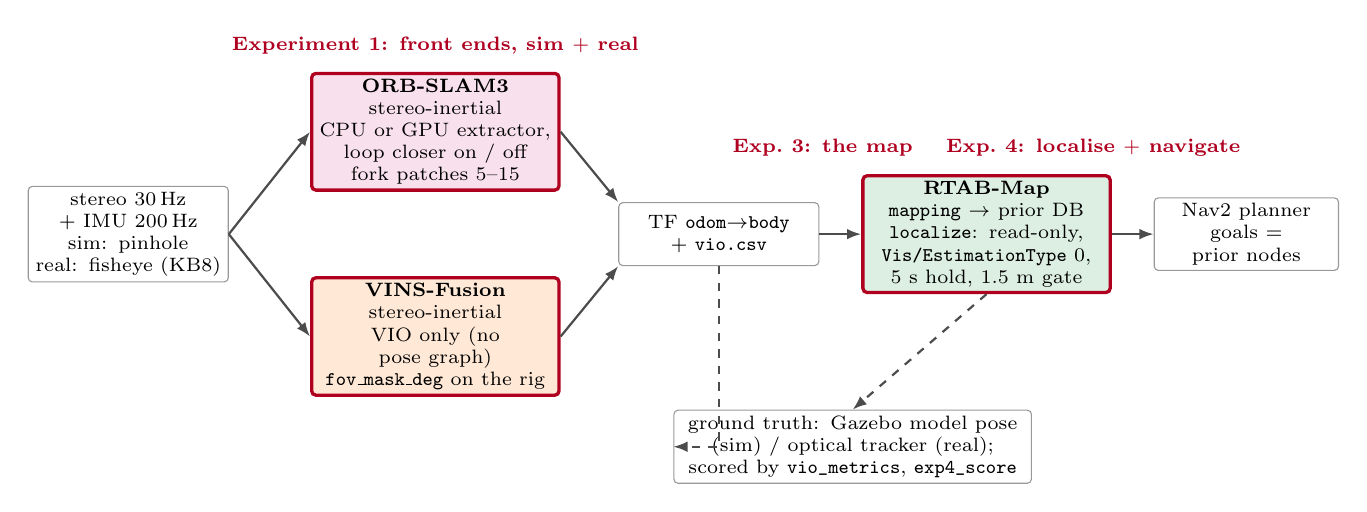
\begin{tikzpicture}
    \node[io, text width=24mm] at (0,0) (sens) {stereo \SI{30}{\hertz}\\$+$ IMU \SI{200}{\hertz}\\sim: pinhole\\real: fisheye (KB8)};
    \node[hotblk, fill=stageorb, text width=30mm] at (3.9,1.3) (orb) {\textbf{ORB-SLAM3} stereo-inertial\\CPU or GPU extractor,\\loop closer on / off\\fork patches 5--15};
    \node[hotblk, fill=stagevins, text width=30mm] at (3.9,-1.3) (vins) {\textbf{VINS-Fusion} stereo-inertial\\VIO only (no pose graph)\\\texttt{fov\_mask\_deg} on the rig};
    \node[io, text width=24mm] at (7.5,0) (tf) {TF \texttt{odom}$\to$\texttt{body}\\$+$ \repo{vio.csv}};
    \node[hotblk, fill=stagertab, text width=30mm] at (10.9,0) (rtab) {\textbf{RTAB-Map}\\\texttt{mapping} $\rightarrow$ prior DB\\\texttt{localize}: read-only,\\\texttt{Vis/EstimationType} 0,\\5 s hold, 1.5 m gate};
    \node[io, text width=22mm] at (14.2,0) (nav) {Nav2 planner\\goals $=$ prior nodes};
    \node[io, text width=44mm] at (9.2,-2.7) (gt) {ground truth: Gazebo model pose (sim) / optical tracker (real); scored by \repo{vio_metrics}, \repo{exp4_score}};
    \draw[arr] (sens.east) -- (orb.west); \draw[arr] (sens.east) -- (vins.west);
    \draw[arr] (orb.east) -- (tf.north west); \draw[arr] (vins.east) -- (tf.south west);
    \draw[arr] (tf) -- (rtab); \draw[arr] (rtab) -- (nav);
    \draw[dasharr] (tf.south) |- (gt.west); \draw[dasharr] (rtab.south) -- (gt.north);
    \node[font=\scriptsize\bfseries, text=hot, above=1mm of orb] {Experiment 1: front ends, sim $+$ real};
    \node[font=\scriptsize\bfseries, text=hot, above=1mm of rtab] {Exp.~3: the map \quad Exp.~4: localise $+$ navigate};
  \end{tikzpicture}}
  \par\vspace{0.4em}
  \scriptsize
  \begin{columns}[T]
    \column{0.5\textwidth}
      \begin{itemize}
        \item Both front ends publish the same thing: a body pose on TF. The
              back end does not know which one is running.
        \item The Atlas, the loop closer and the IMU initialisation of
              slides~5--7 all sit \emph{inside} the ORB-SLAM3 box;
              Experiment~1 switches only the closer and the extractor.
      \end{itemize}
    \column{0.5\textwidth}
      \begin{itemize}
        \item RTAB-Map's own visual odometry (F2M/F2F) is not used; the
              paper's point that the back end is odometry-agnostic is what
              makes the two-front-end comparison fair.
        \item The YOLO masking arm exists in both front ends but is not
              reported in this deck.
      \end{itemize}
  \end{columns}
  \src{Chapter~3 of the report; \repo{vslam_navigation} launch files; \repo{config/wil_sim/stereo_imu.yaml}, \repo{config/wil/stereo_imu.yaml}}
\end{frame}

% ===================================================================== Part 1
\section{What a visual-SLAM system is made of}

\begin{frame}{2. Every system here is a front end, a back end and a map, joined by loop closure}
  \centering
  \resizebox{\textwidth}{!}{%
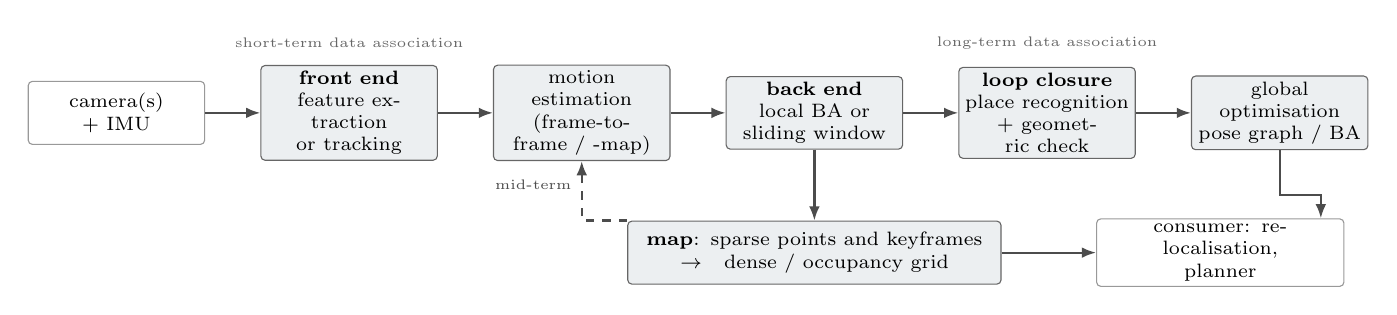
\begin{tikzpicture}[node distance=5mm and 7mm]
    \node[io] (sens) {camera(s)\\$+$ IMU};
    \node[blk, right=of sens] (fe) {\textbf{front end}\\feature extraction\\or tracking};
    \node[blk, right=of fe] (mo) {motion\\estimation\\(frame-to-frame / -map)};
    \node[blk, right=of mo] (be) {\textbf{back end}\\local BA or\\sliding window};
    \node[blk, right=of be] (lc) {\textbf{loop closure}\\place recognition\\$+$ geometric check};
    \node[blk, right=of lc] (go) {global\\optimisation\\pose graph / BA};
    \node[blk, below=9mm of be, text width=46mm] (map) {\textbf{map}: sparse points and keyframes\quad$\rightarrow$\quad dense / occupancy grid};
    \node[io, right=12mm of map, text width=30mm] (use) {consumer: relocalisation,\\planner};
    \draw[arr] (sens) -- (fe);
    \draw[arr] (fe) -- (mo);
    \draw[arr] (mo) -- (be);
    \draw[arr] (be) -- (lc);
    \draw[arr] (lc) -- (go);
    \draw[arr] (be) -- (map);
    \draw[arr] (go.south) |- ($(use.north east)+(-3mm,3mm)$) -- ($(use.north east)+(-3mm,0)$);
    \draw[arr] (map) -- (use);
    \draw[dasharr] (map.north west) -| node[pos=0.8, left, font=\tiny]{mid-term} (mo.south);
    % data-association brackets
    \node[font=\tiny, text=black!60, above=1mm of fe] {short-term data association};
    \node[font=\tiny, text=black!60, above=1mm of lc] {long-term data association};
  \end{tikzpicture}}
  \par\vspace{0.5em}
  \scriptsize
  \begin{columns}[T]
    \column{0.48\textwidth}
      \begin{itemize}
        \item \textbf{Short-term}: match against the last few seconds. Pure VO;
              drift never stops.
        \item \textbf{Mid-term}: match against nearby map points whose drift is
              still small; zero drift in mapped areas.
        \item \textbf{Long-term}: place recognition regardless of drift: loop
              detection, relocalisation, map merging.
      \end{itemize}
    \column{0.48\textwidth}
      \begin{itemize}
        \item ORB-SLAM3 uses all three and adds multi-map.
        \item VINS-Mono is short-term VIO plus long-term loop closure; no
              mid-term reuse.
        \item RTAB-Map is the long-term block alone, fed by whatever odometry
              you give it, plus the occupancy grid the planner needs.
      \end{itemize}
  \end{columns}
  \src{\paper{Campos et al., ORB-SLAM3, IEEE T-RO 2021, §I (three kinds of data association)};
       \paper{Labbé \& Michaud, RTAB-Map, J.\ Field Robotics 2019, §3}}
\end{frame}

% ===================================================================== Part 2
\section{ORB-SLAM3}

\begin{frame}{3. ORB-SLAM3: three threads on one Atlas, every stage reuses the map}
  \centering
  \resizebox{\textwidth}{!}{%
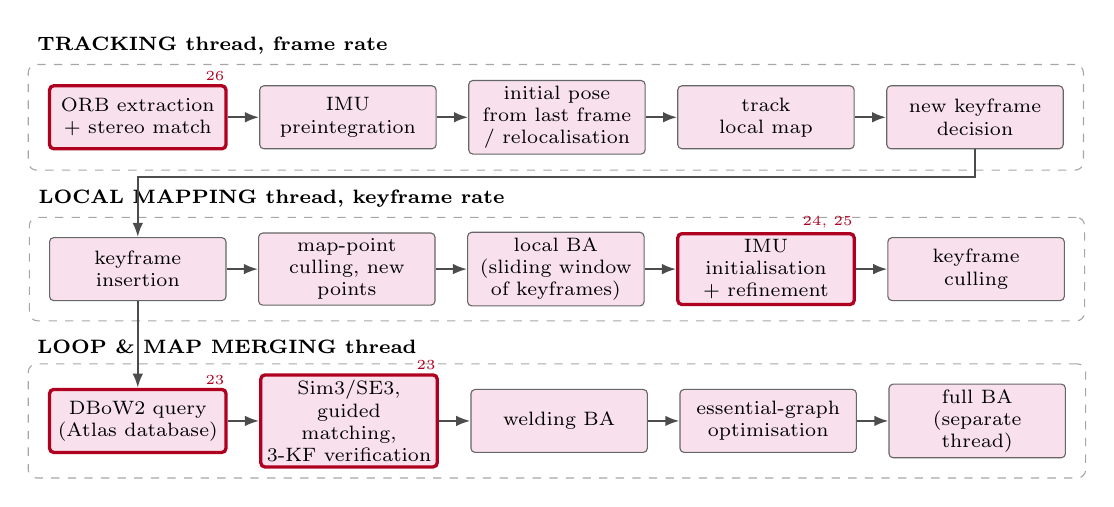
\begin{tikzpicture}[node distance=3mm and 4mm]
    % tracking row
    \node[hotblk, fill=stageorb] (ext) {ORB extraction\\$+$ stereo match};
    \node[pin] at (ext.north east) {26};
    \node[blk, fill=stageorb, right=of ext] (imu) {IMU\\preintegration};
    \node[blk, fill=stageorb, right=of imu] (pred) {initial pose\\from last frame\\/ relocalisation};
    \node[blk, fill=stageorb, right=of pred] (tlm) {track\\local map};
    \node[blk, fill=stageorb, right=of tlm] (kfd) {new keyframe\\decision};
    % local mapping row
    \node[blk, fill=stageorb, below=11mm of ext] (kfi) {keyframe\\insertion};
    \node[blk, fill=stageorb, right=of kfi] (cull) {map-point\\culling, new\\points};
    \node[blk, fill=stageorb, right=of cull] (lba) {local BA\\(sliding window\\of keyframes)};
    \node[hotblk, fill=stageorb, right=of lba] (init) {IMU\\initialisation\\$+$ refinement};
    \node[pin] at (init.north east) {24, 25};
    \node[blk, fill=stageorb, right=of init] (kfc) {keyframe\\culling};
    % loop row
    \node[hotblk, fill=stageorb, below=11mm of kfi] (db) {DBoW2 query\\(Atlas database)};
    \node[pin] at (db.north east) {23};
    \node[hotblk, fill=stageorb, right=of db] (geo) {Sim3/SE3,\\guided matching,\\3-KF verification};
    \node[pin] at (geo.north east) {23};
    \node[blk, fill=stageorb, right=of geo] (weld) {welding BA};
    \node[blk, fill=stageorb, right=of weld] (eg) {essential-graph\\optimisation};
    \node[blk, fill=stageorb, right=of eg] (fba) {full BA\\(separate thread)};
    % groups
    \begin{scope}[on background layer]
      \node[grp, fit=(ext)(kfd), label={[grplbl]north west:TRACKING thread, frame rate}] {};
      \node[grp, fit=(kfi)(kfc), label={[grplbl]north west:LOCAL MAPPING thread, keyframe rate}] {};
      \node[grp, fit=(db)(fba), label={[grplbl]north west:LOOP \& MAP MERGING thread}] {};
    \end{scope}
    \draw[arr] (ext) -- (imu); \draw[arr] (imu) -- (pred); \draw[arr] (pred) -- (tlm); \draw[arr] (tlm) -- (kfd);
    \draw[arr] (kfd.south) -- ++(0,-3.5mm) -| (kfi.north);
    \draw[arr] (kfi) -- (cull); \draw[arr] (cull) -- (lba); \draw[arr] (lba) -- (init); \draw[arr] (init) -- (kfc);
    \draw[arr] (kfi.south) -- ++(0,-3.5mm) -| (db.north);
    \draw[arr] (db) -- (geo); \draw[arr] (geo) -- (weld); \draw[arr] (weld) -- (eg); \draw[arr] (eg) -- (fba);
  \end{tikzpicture}}
  \par\vspace{0.3em}
  \scriptsize
  \begin{itemize}
    \item \textbf{Atlas}: one active map the tracker localises in, plus non-active
          maps; one DBoW2 keyframe database over all of them. Lost for more
          than \SI{5}{\second} $\rightarrow$ a new active map; a revisit merges it back.
    \item Tracking optimises only the last two frames with map points fixed;
          local mapping runs BA on a keyframe window plus fixed covisible
          ones. Red outline: blocks Experiment~1 pins a finding to, with the slide number.
  \end{itemize}
  \src{\paper{Campos et al., ORB-SLAM3, IEEE T-RO 2021, Fig.~1 and §III}}
\end{frame}

\begin{frame}{3. The inertial state is initialised as a MAP problem in three steps, then the map is rotated to gravity}
  \begin{columns}[T]
    \column{0.55\textwidth}
      \scriptsize
      \begin{enumerate}
        \item \textbf{Vision-only MAP}: run pure visual SLAM for about
              \SI{2}{\second}, inserting keyframes at \SI{4}{\hertz}, until
              $k=10$ keyframes exist; visual-only BA gives an up-to-scale
              trajectory $\bar T_{0:k}$.
        \item \textbf{Inertial-only MAP}: hold the trajectory fixed and solve
              for $Y_k=\{s,\,\mathbf R_{wg},\,\mathbf b,\,\bar{\mathbf v}_{0:k}\}$
              from the preintegration residuals plus a prior
              $\lVert\mathbf b\rVert^2_{\Sigma_b^{-1}}$ pulling the biases to
              zero. Gravity is parameterised by two angles about the
              horizontal axes. \emph{Stereo-inertial fixes $s=1$.}
        \item \textbf{Visual-inertial MAP}: joint BA; then the map is scaled
              and \textbf{rotated so that $z$ follows the estimated gravity};
              visual-inertial BA again at 5 and \SI{15}{\second}.
      \end{enumerate}
      Afterwards the map is ``mature''. Where slow motion gives poor
      observability of the inertial parameters, a scale-and-gravity
      refinement runs every \SI{10}{\second} until 100 keyframes or
      \SI{75}{\second}.
    \column{0.45\textwidth}
      \scriptsize
      \textbf{Robustness to tracking loss}
      \begin{itemize}
        \item Visually lost = fewer than 15 map points tracked.
        \item \emph{Short-term lost}: predict the body state from the IMU,
              project map points, search in a large window. Up to
              \SI{5}{\second}.
        \item \emph{Long-term lost}: start a new visual-inertial map; it
              becomes the active map.
        \item A map lost within \SI{15}{\second} of IMU initialisation is
              discarded.
      \end{itemize}
      \vspace{0.6em}
      \textbf{Why this matters later}
      \begin{itemize}
        \item The rotation to gravity is a frame change in the published
              pose (slide 25).
        \item ``Poor observability under slow motion'' is a robot on a flat
              floor (slide 24).
        \item The discard-and-restart heuristics are tuned for a hand-held
              or flying sensor (slide 31).
      \end{itemize}
  \end{columns}
  \src{\paper{Campos et al., ORB-SLAM3, IEEE T-RO 2021, §V-B (IMU initialisation), §V-D (tracking loss)}}
\end{frame}

\begin{frame}{3. Place recognition trades the DBoW2 temporal check for geometric checks that are already in the map}
  \begin{columns}[T]
    \column{0.52\textwidth}
      \scriptsize
      For every new keyframe $K_a$:
      \begin{enumerate}
        \item \textbf{DBoW2 candidates}: the three most similar keyframes in
              the whole Atlas, excluding covisible ones.
        \item \textbf{Local window} around each candidate $K_m$: its
              covisible keyframes and their map points.
        \item \textbf{3D alignment} $T_{am}$ by RANSAC + Horn on 3D--3D
              matches: $Sim(3)$ while the map is not mature, $SE(3)$ after.
        \item \textbf{Guided matching} and non-linear refinement of $T_{am}$
              with a Huber kernel, twice.
        \item \textbf{Verification in three covisible keyframes} of the
              \emph{active} map, instead of waiting for the bag of words to
              fire three times in a row.
        \item \textbf{Gravity check} (inertial, mature map): pitch and roll of
              $T_{am}$ below a threshold.
      \end{enumerate}
      Same area in the active map $\rightarrow$ loop correction; another
      map $\rightarrow$ merge. Both: welding BA in a window, then
      essential-graph optimisation, then (loop) a full BA.
    \column{0.48\textwidth}
      \scriptsize
      \textbf{What the paper gives up to get recall}
      \begin{itemize}
        \item Raw DBoW2 queries reach 50--80\,\% precision and recall; the
              temporal-consistency check moves that to \SI{100}{\percent}
              precision at 30--40\,\% recall and delays every closure by three
              keyframes.
        \item ORB-SLAM3 drops that delay. Its guard against false positives
              is \emph{geometric}: enough matched points agreeing on one
              rigid transform, in three views.
        \item A guard built from point agreement cannot tell two
              \emph{identical} objects apart. That is the warehouse case
              (slide 23).
        \item The gravity check only constrains pitch and roll. A false match
              one aisle over, on a flat floor, passes it (slide 23).
      \end{itemize}
  \end{columns}
  \src{\paper{Campos et al., ORB-SLAM3, IEEE T-RO 2021, §VI-A (place recognition), §VI-B--D (merging and loop closing)}}
\end{frame}

% ===================================================================== Part 3
\section{VINS}

\begin{frame}{4. VINS-Mono: preprocessing, initialisation, sliding-window VIO, relocalisation, 4-DoF pose graph}
  \centering
  \resizebox{\textwidth}{!}{%
  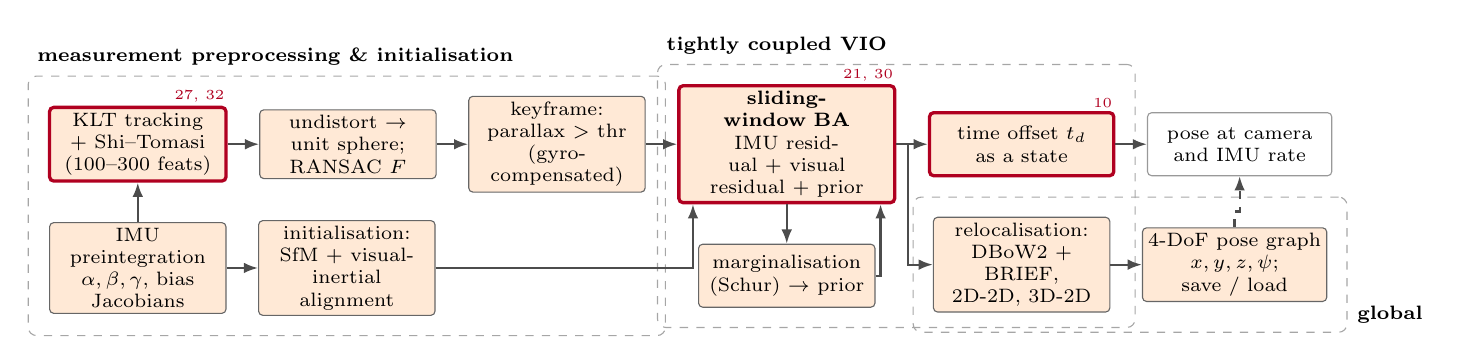
\begin{tikzpicture}[node distance=3mm and 4mm]
    \node[hotblk, fill=stagevins] (klt) {KLT tracking\\$+$ Shi--Tomasi\\(100--300 feats)};
    \node[pin] at (klt.north east) {27, 32};
    \node[blk, fill=stagevins, right=of klt] (ransac) {undistort $\rightarrow$\\unit sphere;\\RANSAC $F$};
    \node[blk, fill=stagevins, right=of ransac] (kf) {keyframe:\\parallax $>$ thr\\(gyro-compensated)};
    \node[blk, fill=stagevins, below=5mm of klt] (pre) {IMU\\preintegration\\$\alpha,\beta,\gamma$, bias Jacobians};
    \node[blk, fill=stagevins, right=of pre] (ini) {initialisation:\\SfM $+$ visual-\\inertial alignment};
    \node[hotblk, fill=stagevins, right=of kf, text width=26mm] (win) {\textbf{sliding-window BA}\\IMU residual $+$ visual\\residual $+$ prior};
    \node[pin] at (win.north east) {21, 30};
    \node[blk, fill=stagevins, below=5mm of win] (marg) {marginalisation\\(Schur) $\rightarrow$ prior};
    \node[hotblk, fill=stagevins, right=of win, text width=22mm] (td) {time offset $t_d$\\as a state};
    \node[pin] at (td.north east) {10};
    \node[blk, fill=stagevins, below=5mm of td] (relo) {relocalisation:\\DBoW2 $+$ BRIEF,\\2D-2D, 3D-2D};
    \node[blk, fill=stagevins, right=of relo, text width=22mm] (pg) {4-DoF pose graph\\$x,y,z,\psi$; save / load};
    \node[io, right=of td, text width=22mm] (out) {pose at camera\\and IMU rate};
    \begin{scope}[on background layer]
      \node[grp, fit=(klt)(kf)(pre)(ini), label={[grplbl]north west:measurement preprocessing \& initialisation}] {};
      \node[grp, fit=(win)(marg)(td), label={[grplbl]north west:tightly coupled VIO}] {};
      \node[grp, fit=(relo)(pg), label={[grplbl]south east:global}] {};
    \end{scope}
    \draw[arr] (klt) -- (ransac); \draw[arr] (ransac) -- (kf); \draw[arr] (kf) -- (win);
    \draw[arr] (pre) -- (ini); \draw[arr] (ini.east) -| ($(win.south west)+(2mm,0)$);
    \draw[arr] (pre.north) -- (klt.south);
    \draw[arr] (win.south) -- (marg.north); \draw[arr] (marg.east) -| ($(win.south east)+(-2mm,0)$);
    \draw[arr] (win) -- (td); \draw[arr] (td) -- (out);
    \draw[arr] (win.east) -- ++(1.5mm,0) |- (relo.west);
    \draw[arr] (relo) -- (pg);
    \draw[dasharr] (pg.north) -- ++(0,2mm) -| (out.south);
  \end{tikzpicture}}
  \par\vspace{0.3em}
  \scriptsize
  \begin{itemize}
    \item The window holds $n$ IMU states $\{p,v,q,b_a,b_g\}$, the camera--IMU
          extrinsic, and $m$ features as inverse depth; Ceres minimises prior
          $+$ IMU $+$ visual (Huber) residuals.
    \item Roll and pitch are observable from gravity, so drift lives in
          $x,y,z,\psi$ only: the pose graph is 4-DoF. Sequential edges from VIO,
          loop edges from relocalisation, Huber on loop edges only.
    \item In our fork the pose graph is not run: VINS-Fusion here is the VIO
          block, short-term data association only (slide 21).
  \end{itemize}
  \src{\paper{Qin, Li \& Shen, VINS-Mono, IEEE T-RO 2018, Fig.~2, §IV--VIII}}
\end{frame}

\begin{frame}{4. The window is bounded by marginalisation, and the visual residual lives on the unit sphere}
  \begin{columns}[T]
    \column{0.5\textwidth}
      \scriptsize
      \textbf{Marginalisation (Fig.~7 of the paper)}
      \begin{itemize}
        \item If the second-latest frame is a keyframe, the \emph{oldest}
              frame and its measurements are marginalised into a prior (Schur
              complement).
        \item If it is not a keyframe, its visual measurements are dropped
              but its IMU preintegration is kept and continued to the next
              frame, so the system stays sparse and keyframes stay spatially
              separated.
        \item Cost: linearisation points are fixed early. The authors accept
              the suboptimality because ``small drifting is acceptable for
              VIO''.
      \end{itemize}
      \textbf{Keyframe criteria}: average parallax above a threshold with
      short-term gyro integration removing rotation-only parallax; or tracked
      features below a threshold.
    \column{0.5\textwidth}
      \scriptsize
      \textbf{Visual residual}
      \begin{itemize}
        \item Defined on a \emph{unit sphere}, not an image plane, so that
              wide-angle, fisheye and omnidirectional cameras fit the same
              formulation; the 2-DoF residual is projected onto the tangent
              plane.
        \item Features are tracked by KLT, ``slightly more robust than
              descriptor matching'' for tracking, but with no descriptors
              there is no mid-term reuse of map points.
      \end{itemize}
      \textbf{Consequences for Part B}
      \begin{itemize}
        \item A bounded window with no map to fall back on means the error
              is smooth drift, never a jump (slide 21), and a texture dip is
              paid for directly (slide 27).
        \item The stereo build we run keeps the unit-sphere residual behind
              a compile flag and divides by $z$ in the tracker (slide 32).
        \item Bounded state $\Rightarrow$ bounded memory, at the cost of
              solving a dense problem every frame (slide 30).
      \end{itemize}
  \end{columns}
  \src{\paper{Qin, Li \& Shen, VINS-Mono, IEEE T-RO 2018, §IV-A, §VI-C, §VI-D}}
\end{frame}

\begin{frame}{4. The camera--IMU time offset is a state: shift the feature, not the stream}
  \begin{columns}[T]
    \column{0.55\textwidth}
      \scriptsize
      \begin{itemize}
        \item Triggering delay, transmission delay and unsynchronised clocks
              make $t_{\mathrm{IMU}} = t_{\mathrm{cam}} + t_d$ with $t_d$
              unknown; a few to hundreds of milliseconds on self-assembled
              rigs.
        \item Over a few milliseconds the camera moves at constant speed, so
              a feature moves at constant velocity
              $V_l^k = (z_l^{k+1}-z_l^k)/(t_{k+1}-t_k)$ on the image plane.
        \item The reprojection residual is rewritten with the observation
              shifted: $z_l^k(t_d) = [u_l^k\;v_l^k]^\top + t_d V_l^k$, and
              $t_d$ joins the state vector of the sliding-window BA.
        \item After each solve the subsequent camera timestamps are
              compensated and the estimator continues on the residual
              $\delta t_d$, coarse to fine.
      \end{itemize}
      \textbf{Measured in the paper}: without calibration VINS-Mono's RMSE on
      MH03 follows a parabola in $t_d$ and tolerates only about
      \SI{6}{\milli\second}; with it the RMSE is flat from $-40$ to
      \SI{+40}{\milli\second}. The estimate converges in a few seconds; the
      RealSense ZR300 offset was \SI{12.74}{\milli\second} and scaled with
      exposure time (slope about 0.5).
    \column{0.45\textwidth}
      \scriptsize
      \textbf{Why it is in this deck}
      \begin{itemize}
        \item Our real rig is exactly the paper's case: a RealSense IMU and
              separate fisheye cameras, timestamped by the host.
        \item The sim has an exact clock, so every simulation result in Part B
              is at $t_d=0$ by construction.
        \item On the real rig the td handling in the node was one of two
              defects fixed this month, before the field-of-view fault was
              found (slide 32). Nothing in Part B isolates its size yet.
      \end{itemize}
      \vspace{0.6em}
  \end{columns}
  \src{\paper{Qin \& Shen, Online Temporal Calibration for Monocular Visual-Inertial Systems, IROS 2018, §III, Fig.~7, Fig.~9}}
\end{frame}

% ===================================================================== Part 4
\section{RTAB-Map}

\begin{frame}{5. RTAB-Map is the long-term block alone: odometry comes in on TF, a grid and a correction come out}
  \centering
  \resizebox{\textwidth}{!}{%
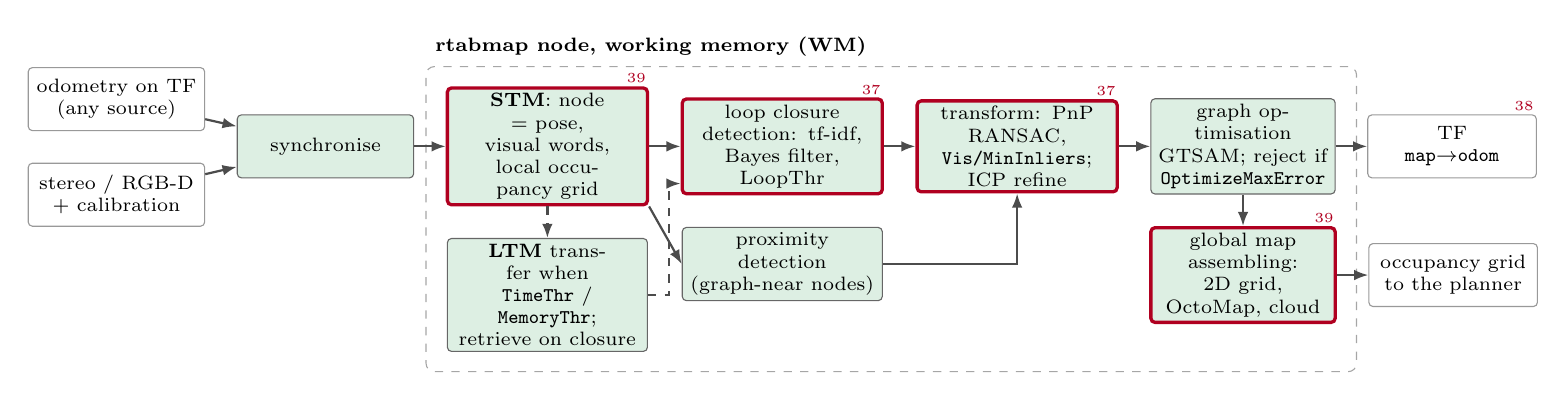
\begin{tikzpicture}[node distance=3mm and 4mm]
    \node[io] (odom) {odometry on TF\\(any source)};
    \node[io, below=4mm of odom] (cam) {stereo / RGB-D\\$+$ calibration};
    \node[blk, fill=stagertab, right=of odom, yshift=-6mm] (sync) {synchronise};
    \node[hotblk, fill=stagertab, right=of sync, text width=24mm] (stm) {\textbf{STM}: node $=$ pose,\\visual words,\\local occupancy grid};
    \node[pin] at (stm.north east) {39};
    \node[hotblk, fill=stagertab, right=of stm, text width=24mm] (lcd) {loop closure\\detection: tf-idf,\\Bayes filter, LoopThr};
    \node[pin] at (lcd.north east) {37};
    \node[blk, fill=stagertab, below=4mm of lcd, text width=24mm] (prox) {proximity\\detection\\(graph-near nodes)};
    \node[hotblk, fill=stagertab, right=of lcd, text width=24mm] (geo) {transform: PnP\\RANSAC, \texttt{Vis/MinInliers};\\ICP refine};
    \node[pin] at (geo.north east) {37};
    \node[blk, fill=stagertab, right=of geo, text width=22mm] (opt) {graph optimisation\\GTSAM; reject if\\\texttt{OptimizeMaxError}};
    \node[hotblk, fill=stagertab, below=4mm of opt, text width=22mm] (asm) {global map\\assembling: 2D grid,\\OctoMap, cloud};
    \node[pin] at (asm.north east) {39};
    \node[io, right=of opt, text width=20mm] (tf) {TF\\\texttt{map}$\to$\texttt{odom}};
    \node[pin] at (tf.north east) {38};
    \node[io, right=of asm, text width=20mm] (grid) {occupancy grid\\to the planner};
    \node[blk, fill=stagertab, below=4mm of stm, text width=24mm] (ltm) {\textbf{LTM} transfer when\\\texttt{TimeThr} / \texttt{MemoryThr};\\retrieve on closure};
    \begin{scope}[on background layer]
      \node[grp, fit=(stm)(lcd)(prox)(geo)(opt)(asm)(ltm), label={[grplbl]north west:rtabmap node, working memory (WM)}] {};
    \end{scope}
    \draw[arr] (odom) -- (sync); \draw[arr] (cam) -- (sync);
    \draw[arr] (sync) -- (stm); \draw[arr] (stm) -- (lcd); \draw[arr] (stm.south east) -- (prox.west);
    \draw[arr] (lcd) -- (geo); \draw[arr] (prox.east) -| ($(geo.south)+(0,0)$);
    \draw[arr] (geo) -- (opt); \draw[arr] (opt) -- (asm); \draw[arr] (opt) -- (tf); \draw[arr] (asm) -- (grid);
    % Retrieval from LTM: routed up the clear 4 mm corridor between the
    % stm/ltm and lcd/prox columns, so it does not cross the proximity box.
    \draw[dasharr] (stm) -- (ltm);
    \draw[dasharr] (ltm.east) -| ($(lcd.south west)+(-1.5mm,1.5mm)$) -- ++(1.5mm,0);
  \end{tikzpicture}}
  \par\vspace{0.3em}
  \scriptsize
  \begin{itemize}
    \item A node is created at \texttt{Rtabmap/DetectionRate}; its local grid
          is built once, in the robot frame, from depth or disparity and placed
          in the world by the graph pose. A loop closure re-assembles the
          global grid from all node poses.
    \item Loop closure is appearance-only and visual; the geometric check is the
          \emph{same} PnP motion estimation as the visual odometry. A third guard
          rejects closures whose optimised link moved more than
          \texttt{RGBD/OptimizeMaxError} times its variance.
    \item Localisation mode: the graph is read-only, and the output is the
          \texttt{map}$\to$\texttt{odom} correction; between accepted fixes the
          published pose is the odometry's dead reckoning.
  \end{itemize}
  \src{\paper{Labbé \& Michaud, RTAB-Map, J.\ Field Robotics 2019, Fig.~1, §3.3--3.6}}
\end{frame}

\begin{frame}{5. Accepting one fix takes two stages, because they answer two different questions}
  \centering
  \resizebox{\textwidth}{!}{%
  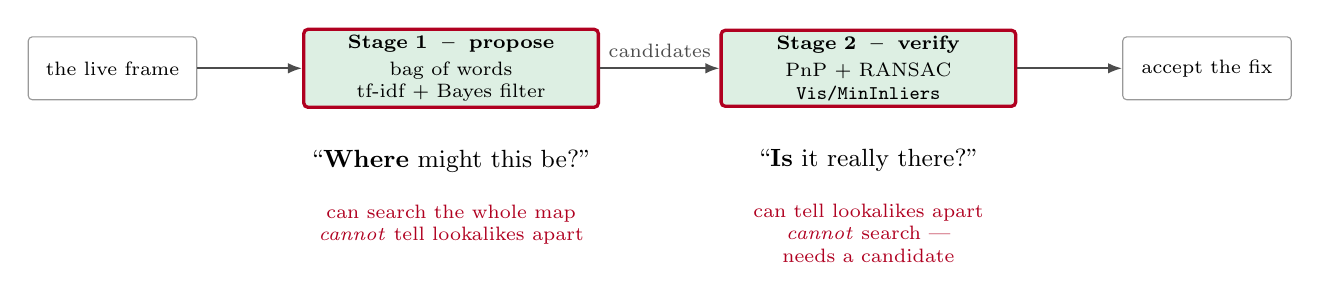
\begin{tikzpicture}[font=\small]
    \node[io, text width=20mm] at (0,0) (frame) {the live frame};
    \node[hotblk, fill=stagertab, text width=36mm] at (4.3,0) (s1)
      {\textbf{Stage 1 \;--\; propose}\\[2pt] bag of words\\ tf-idf $+$ Bayes filter};
    \node[hotblk, fill=stagertab, text width=36mm] at (9.6,0) (s2)
      {\textbf{Stage 2 \;--\; verify}\\[2pt] PnP $+$ RANSAC\\ \texttt{Vis/MinInliers}};
    \node[io, text width=20mm] at (13.9,0) (fix) {accept the fix};
    \draw[arr] (frame) -- (s1);
    \draw[arr] (s1) -- node[above, font=\scriptsize]{candidates} (s2);
    \draw[arr] (s2) -- (fix);
    \node[font=\small, below=4mm of s1, text width=40mm, align=center]
      {``\textbf{Where} might this be?''};
    \node[font=\small, below=4mm of s2, text width=40mm, align=center]
      {``\textbf{Is} it really there?''};
    \node[font=\scriptsize, text=hot, below=11mm of s1, text width=42mm, align=center]
      {can search the whole map\\ \emph{cannot} tell lookalikes apart};
    \node[font=\scriptsize, text=hot, below=11mm of s2, text width=42mm, align=center]
      {can tell lookalikes apart\\ \emph{cannot} search --- needs a candidate};
  \end{tikzpicture}}
  \par\vspace{1.2em}
  \small No single method does both jobs. The next three slides are why, and
  what each one costs.
  \src{\paper{Labbé \& Michaud 2019, §3.4}}
\end{frame}

\begin{frame}{5. Stage 1 throws the geometry away, because searching everywhere is otherwise unaffordable}
  \begin{columns}[T]
    \column{0.44\textwidth}
      \small
      \textbf{The cost of asking ``where?'' honestly}
      \par\vspace{0.4em}
      \begin{tabular}{lr}
        \toprule
        nodes in the U prior & 148 \\
        features per node & 888 \\
        \midrule
        compare one frame\\ against every node & $\approx\!10^{8}$ \\
        & \scriptsize descriptor comparisons \\
        \bottomrule
      \end{tabular}
      \par\vspace{0.8em}
      \small …every single detection cycle. That is why the search stage
      cannot look at geometry at all.
    \column{0.56\textwidth}
      \small
      \textbf{What it does instead}
      \begin{itemize}
        \item \textbf{A bag of words}: forget \emph{where} the features were,
              keep only \emph{which} words appeared, and look them up in an
              inverted index. Cost barely grows with the map.
        \item \textbf{tf-idf}: words are not equally useful. A shelf edge is
              in every frame and says nothing; a rare word actually locates
              you. In a warehouse of repeated structure this is what carries
              the signal.
        \item \textbf{A Bayes filter}: one frame is not evidence. It
              accumulates across frames, only allows moves to nearby places,
              and keeps a \emph{virtual place} meaning ``nowhere I know'' ---
              so the answer is a probability over places, not a single guess.
      \end{itemize}
  \end{columns}
  \src{Counts measured from the prior \repo{.db}; \paper{Labbé \& Michaud 2019, §3.4}}
\end{frame}

\begin{frame}{5. The two stages cannot be merged, and our own runs show it in both directions}
  \begin{columns}[T]
    \column{0.5\textwidth}
      \small
      \textbf{Remove stage 2}
      \par\vspace{0.3em}
      \bad{64 of 346} proposals had \emph{zero} features in geometric
      agreement --- and carried a median of \textbf{77 matching words}.
      \par\vspace{0.4em}
      Without the geometry those all become fixes. The retired ungated
      configuration is what that looks like: two runs over a metre for
      \SI{36}{} and \SI{23.5}{\second}, as far as \SI{6.80}{\metre}, the pose
      cutting through three shelf rows.
    \column{0.5\textwidth}
      \small
      \textbf{Make stage 1 strict enough to replace stage 2}
      \par\vspace{0.3em}
      \texttt{Vis/MinInliers} 35 plus the distribution test, swept 11--12
      November: \bad{0 of 81 poses} localised on one recording.
      \par\vspace{0.4em}
      It keeps the lookalikes out and the honest fixes with them. The two
      stages fail in \emph{opposite} directions, which is exactly why both
      have to exist.
  \end{columns}
  \par\vspace{1.0em}
  \centering
  \small \textbf{In one line}: stage 1 discards information so that it can
  search; stage 2 puts it back so that it can decide.
  \src{\repo{script/exp4_rtabmap_gating.py}; acceptance sweep of 11--12 November}
\end{frame}

\begin{frame}{5. Four gates stand between a camera frame and a graph node}
  \centering
  \resizebox{\textwidth}{!}{%
  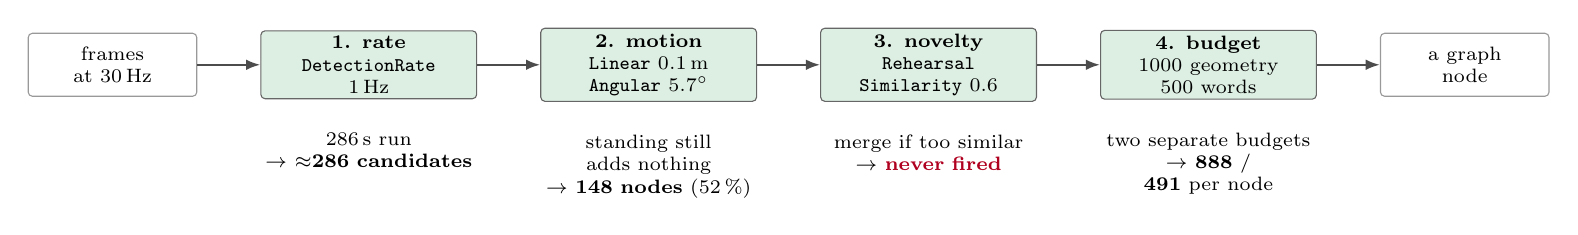
\begin{tikzpicture}[font=\scriptsize, node distance=4mm]
    \node[io, text width=20mm] (f) {frames\\ at \SI{30}{\hertz}};
    \node[blk, fill=stagertab, text width=26mm, right=8mm of f] (g1)
      {\textbf{1. rate}\\ \texttt{DetectionRate}\\ \SI{1}{\hertz}};
    \node[blk, fill=stagertab, text width=26mm, right=8mm of g1] (g2)
      {\textbf{2. motion}\\ \texttt{Linear} \SI{0.1}{\metre}\\ \texttt{Angular} \SI{5.7}{\degree}};
    \node[blk, fill=stagertab, text width=26mm, right=8mm of g2] (g3)
      {\textbf{3. novelty}\\ \texttt{Rehearsal}\\ \texttt{Similarity} 0.6};
    \node[blk, fill=stagertab, text width=26mm, right=8mm of g3] (g4)
      {\textbf{4. budget}\\ 1000 geometry\\ 500 words};
    \node[io, text width=20mm, right=8mm of g4] (n) {a graph\\ node};
    \draw[arr] (f) -- (g1); \draw[arr] (g1) -- (g2); \draw[arr] (g2) -- (g3);
    \draw[arr] (g3) -- (g4); \draw[arr] (g4) -- (n);
    \node[font=\scriptsize, below=3mm of g1, text width=28mm, align=center]
      {\SI{286}{\second} run\\ $\rightarrow$ \textbf{$\approx$286 candidates}};
    \node[font=\scriptsize, below=3mm of g2, text width=28mm, align=center]
      {standing still adds nothing\\ $\rightarrow$ \textbf{148 nodes} (52\,\%)};
    \node[font=\scriptsize, below=3mm of g3, text width=28mm, align=center]
      {merge if too similar\\ $\rightarrow$ \hotmark{never fired}};
    \node[font=\scriptsize, below=3mm of g4, text width=28mm, align=center]
      {two separate budgets\\ $\rightarrow$ \textbf{888} / \textbf{491} per node};
  \end{tikzpicture}}
  \par\vspace{0.9em}
  \begin{columns}[T]
    \column{0.48\textwidth}
      \small
      \begin{itemize}
        \item Nodes end up a median \SI{2.67}{\metre} apart
              (\SIrange{0.15}{5.40}{\metre}).
        \item ``Never fired'' is measured: all 148 nodes carry weight 0, so
              every node that passed gate~2 was different enough to keep.
      \end{itemize}
    \column{0.52\textwidth}
      \small
      \begin{itemize}
        \item \textbf{The two budgets matter.} Of 888 features kept per node,
              only $\approx$491 become vocabulary \emph{words} (the 500
              ceiling); the other $\approx$400 exist only for stage~2. The bag
              and the geometry are fed separately.
      \end{itemize}
  \end{columns}
  \src{Measured from the prior \repo{.db}: node count, weights, stamps, poses and per-node feature counts}
\end{frame}

\begin{frame}{5. The configuration: everything is the library default but two}
  \begin{columns}[T]
    \column{0.46\textwidth}
      \scriptsize
      \resizebox{\textwidth}{!}{%
      \begin{tabular}{llr}
        \toprule
        & Parameter & Ours \\
        \midrule
        \multirow{2}{*}{propose}
          & \texttt{Rtabmap/DetectionRate} & \SI{1.0}{\hertz} \\
          & \texttt{Rtabmap/LoopThr} & 0.11 \\
        \multirow{5}{*}{node}
          & \texttt{RGBD/LinearUpdate} & \SI{0.1}{\metre} \\
          & \texttt{RGBD/AngularUpdate} & \SI{0.1}{\radian} \\
          & \texttt{Mem/RehearsalSimilarity} & 0.6 \\
          & \texttt{Kp/MaxFeatures} (words) & 500 \\
          & \texttt{Vis/MaxFeatures} (geom.) & 1000 \\
        \multirow{3}{*}{verify}
          & \texttt{Vis/MinInliers} & 20 \\
          & \texttt{Vis/EstimationType} & \hotmark{0} \\
          & \texttt{Vis/InlierDistance} & \SI{0.1}{\metre} \\
        \multirow{2}{*}{graph}
          & \texttt{RGBD/OptimizeMaxError} & \hotmark{10.0} \\
          & \texttt{Reg/Strategy} & 0 (Vis only) \\
        memory & \texttt{TimeThr} / \texttt{MemoryThr} & 0 / 0 \\
        \multirow{2}{*}{ours}
          & \repo{localize_delay_s} & \SI{5}{\second} \\
          & correction gate & \SI{1.5}{\metre} \\
        \bottomrule
      \end{tabular}}
    \column{0.54\textwidth}
      \small
      \textbf{Only two values depart from RTAB-Map 0.23}
      \begin{itemize}
        \item \texttt{EstimationType} \hotmark{0}: matched points must agree
              \emph{in metres}, not merely reproject.
        \item \texttt{OptimizeMaxError} \hotmark{10}: the default 3.0 rejects
              every closure a drifting VIO proposes.
      \end{itemize}
      \vspace{0.3em}
      \textbf{Two things are \emph{not} running}
      \begin{itemize}
        \item \textbf{Memory management is off} (\texttt{TimeThr},
              \texttt{MemoryThr} 0): no node ever left working memory.
              Harmless at 148 nodes, not as the map grows.
        \item \textbf{The ICP check is off} (\texttt{Reg/Strategy} 2) in all
              six runs --- the one guard that looks at 3-D structure rather
              than at matched points.
      \end{itemize}
      \vspace{0.3em}
      \textbf{And Experiment~4 adds nothing}: read-only runs, so all 148 bags
      come from the mapping run.
  \end{columns}
  \src{Parameters from \repo{exp4/*/launch.log} and \repo{Parameters.h} (rtabmap 0.23)}
\end{frame}

% ===================================================================== Part 6
\section{Nav2}

\begin{frame}{6. Nav2 consumes the localised pose and the prior grid, and nothing else}
  \centering
  \resizebox{\textwidth}{!}{%
  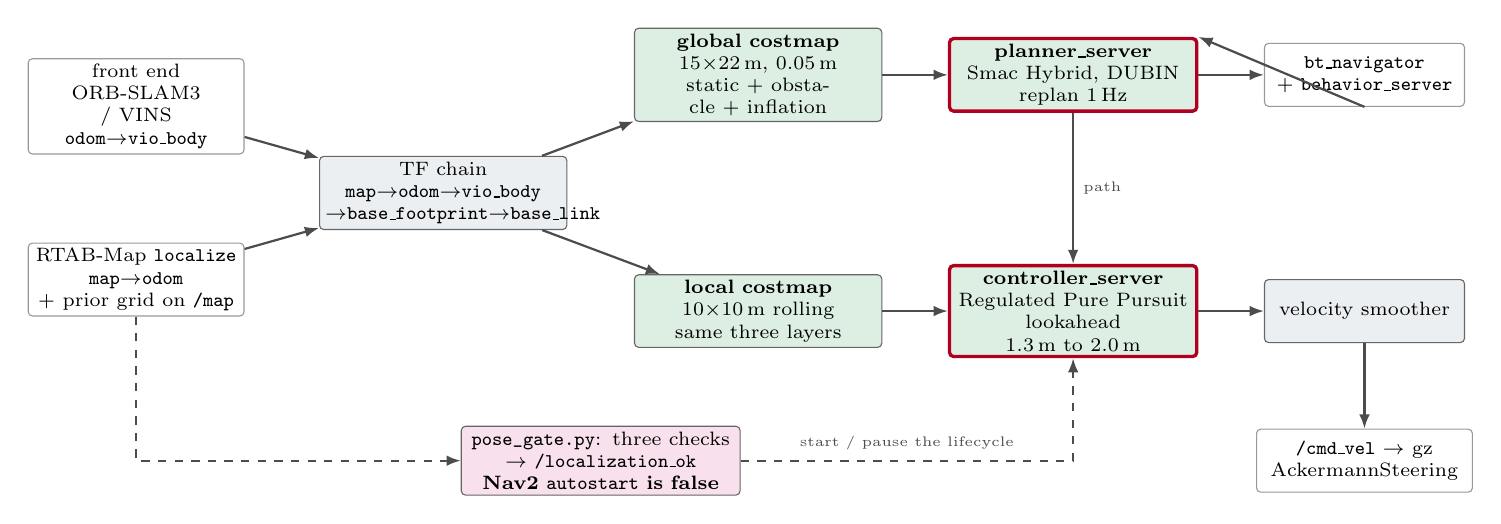
\begin{tikzpicture}[font=\scriptsize]
    % --- inputs
    \node[io, text width=26mm] at (0, 1.1) (fe) {front end\\ ORB-SLAM3 / VINS\\ \texttt{odom}$\to$\texttt{vio\_body}};
    \node[io, text width=26mm] at (0,-1.1) (rt) {RTAB-Map \texttt{localize}\\ \texttt{map}$\to$\texttt{odom}\\ $+$ prior grid on \texttt{/map}};
    % --- what Nav2 actually reads
    \node[blk, text width=30mm] at (3.9, 0) (tf) {TF chain\\ \texttt{map}$\to$\texttt{odom}$\to$\texttt{vio\_body}\\ $\to$\texttt{base\_footprint}$\to$\texttt{base\_link}};
    % --- costmaps
    \node[blk, fill=stagertab, text width=30mm] at (7.9, 1.5) (gc) {\textbf{global costmap}\\ \SI{15}{}$\times$\SI{22}{\metre}, \SI{0.05}{\metre}\\ static $+$ obstacle $+$ inflation};
    \node[blk, fill=stagertab, text width=30mm] at (7.9,-1.5) (lc) {\textbf{local costmap}\\ \SI{10}{}$\times$\SI{10}{\metre} rolling\\ same three layers};
    % --- servers
    \node[hotblk, fill=stagertab, text width=30mm] at (11.9, 1.5) (pl) {\textbf{planner\_server}\\ Smac Hybrid, DUBIN\\ replan \SI{1}{\hertz}};
    \node[hotblk, fill=stagertab, text width=30mm] at (11.9,-1.5) (ct) {\textbf{controller\_server}\\ Regulated Pure Pursuit\\ lookahead \SIrange{1.3}{2.0}{\metre}};
    % --- output
    \node[blk, text width=24mm] at (15.6,-1.5) (vs) {velocity smoother};
    \node[io, text width=24mm] at (15.6, 1.5) (bt) {\texttt{bt\_navigator}\\ $+$ \texttt{behavior\_server}};
    \node[io, text width=26mm] at (15.6,-3.4) (cmd) {\texttt{/cmd\_vel} $\to$ gz\\ AckermannSteering};
    % --- the gate
    \node[blk, fill=stageorb, text width=34mm] at (5.9,-3.4) (pg) {\repo{pose_gate.py}: three checks $\to$ \texttt{/localization\_ok}\\ \textbf{Nav2 \texttt{autostart} is false}};
    \draw[arr] (fe) -- (tf); \draw[arr] (rt) -- (tf);
    \draw[arr] (tf) -- (gc); \draw[arr] (tf) -- (lc);
    \draw[arr] (gc) -- (pl); \draw[arr] (lc) -- (ct);
    \draw[arr] (pl.east) -- (bt.west);
    \draw[arr] (bt.south) -- (pl.north east);
    \draw[arr] (pl.south) -- node[right, font=\tiny]{path} (ct.north);
    \draw[arr] (ct) -- (vs);
    \draw[arr] (vs.south) -- (cmd.north);
    \draw[dasharr] (rt.south) |- (pg.west);
    \draw[dasharr] (pg.east) -| node[pos=0.25, above, font=\tiny]{start / pause the lifecycle} (ct.south);
  \end{tikzpicture}}
  \par\vspace{0.8em}
  \small
  Nav2 never sees ground truth. It is driven entirely by the pose the
  previous five slides produce, on the grid the same database holds --- so
  every error in slides~34--41 arrives here as a planning input.
  \src{\repo{vslam_navigation/launch/navigate_sim.launch.py}, \repo{params/nav2_sim.yaml}, \repo{scripts/pose_gate.py}}
\end{frame}

\begin{frame}{6. The Nav2 configuration follows the chassis, except where SLAM localisation changed the premise}
  \begin{columns}[T]
    \column{0.46\textwidth}
      \scriptsize
      \resizebox{\textwidth}{!}{%
      \begin{tabular}{llr}
        \toprule
        & Parameter & Value \\
        \midrule
        \multirow{3}{*}{chassis}
          & wheel base & \SI{0.42}{\metre} \\
          & steering limit & \SI{35}{\degree} \\
          & min turning radius & \SI{0.75}{\metre} \\
        \multirow{4}{*}{planner}
          & plugin & Smac Hybrid \\
          & motion model & DUBIN \\
          & \texttt{allow\_unknown} & \hotmark{false} \\
          & replan rate & \SI{1.0}{\hertz} \\
        \multirow{4}{*}{controller}
          & plugin & Reg.\ Pure Pursuit \\
          & \texttt{desired\_linear\_vel} & \SI{1.5}{\metre\per\second} \\
          & lookahead & \SIrange{1.3}{2.0}{\metre} \\
          & \texttt{use\_collision\_detection} & \hotmark{false} \\
        \multirow{3}{*}{costmap}
          & global & \SI{15}{}$\times$\SI{22}{\metre} fixed \\
          & local & \hotmark{\SI{10}{}$\times$\SI{10}{\metre} rolling} \\
          & \texttt{inflation\_radius} & \SI{0.80}{\metre} \\
        lifecycle & \texttt{autostart} & \hotmark{false} \\
        \bottomrule
      \end{tabular}}
      \par\vspace{0.5em}
      \scriptsize
      \bad{Collision checking sits with the planner, not the controller.} On,
      a sweep reached ``paralysis, 155 vetoes,
      \SI{0.10}{\metre\per\second}'' --- it vetoes the controller's own
      corner-cutting against the inflation ring. So it will not stop for a
      person it sees: avoidance is the \SI{1}{\hertz} replan.
      \par\vspace{0.2em}
      \bad{Not exercised yet}: all six Experiment~4 runs were hand-driven, no
      goal commanded (slide~34).
    \column{0.54\textwidth}
      \small
      \textbf{Four things differ because the pose comes from SLAM}
      \begin{itemize}
        \item \textbf{The local costmap rolls.} A fixed window in the
              \texttt{odom} frame was safe only while
              \texttt{map}$\to$\texttt{odom} was an exact identity. That
              correction now jumps.
        \item \textbf{\texttt{autostart} false.} \repo{pose_gate.py} starts the
              stack when localisation is sound and pauses it when it is not:
              a low covariance is \emph{not} a correctness signal.
        \item \textbf{\texttt{allow\_unknown} false.} A stereo prior has
              genuinely unseen space, so some goals will be refused rather than
              planned badly.
        \item \textbf{\texttt{transform\_tolerance} \SI{0.30}{\second}}: the
              pose arrives through two nodes at two different rates.
      \end{itemize}
  \end{columns}
  \src{\repo{vslam_navigation/params/nav2_sim.yaml}}
\end{frame}

% ===================================================================== Part 7
\section{Experiment 1, simulation}

\begin{frame}{7. Experiment 1: two families of estimator on the same four recordings, one run per cell}
  \begin{columns}[T]
    \column{0.5\textwidth}
      \scriptsize\setlength{\tabcolsep}{3pt}
      \resizebox{\textwidth}{!}{%
\begin{tabular}{lllrr}
        \toprule
        Recording & Layout & Traffic & Route [m] & Span [s] \\
        \midrule
        \repo{realistic_000} & U & none & 171.3 & 125.5 \\
        \repo{realistic_001} & I & none & 133.0 & 96.9 \\
        \repo{realistic_002} & U & jacks, people & 102.7 & 79.5 \\
        \repo{realistic_003} & I & jacks, people & 158.0 & 117.0 \\
        \bottomrule
      \end{tabular}}
      \par\vspace{0.6em}
      \scriptsize
      \textbf{Non-visual}: wheel odometry, IMU dead reckoning, an EKF at the
      visual systems' \emph{own} inertial noise file (gyro \num{0.002},
      accel \num{0.02}, gyro walk \num{1e-4}), and the same EKF on measured
      noise as a diagnostic.\\[0.4em]
      \textbf{Visual}: VINS-Fusion once; ORB-SLAM3 four times (CPU / GPU
      extractor $\times$ closer on / off). Replay at rate 1.0, live node, no
      detector.
    \column{0.5\textwidth}
      \scriptsize
      \begin{itemize}
        \item Aligned ATE: RMSE after a rigid $SE(3)$ fit, scale fixed, in
              3-D. Ground truth moved from model origin to the IMU point
              (\SI{0.338}{\metre} forward, \SI{0.192}{\metre} up).
        \item RPE at \SI{1}{\second}, over pairs that span no jump.
        \item Closer state read from \repo{loop_closing.csv}, never from the
              run name.
        \item Traffic is a \emph{condition} of a recording, not a tested
              factor: no two recordings share a route.
        \item Cost and repeatability come from 18 extra runs on the two
              mapping bags (3 repeats $\times$ 6 configurations).
      \end{itemize}
      \vspace{0.4em}
      \textbf{Methodology link}: both visual pipelines weight their
      preintegration residual by $\Sigma_I$ built from this same noise file;
      the EKF is handed the same numbers so the three run on one inertial
      model.
  \end{columns}
  \src{\repo{insights/experiment_1/experiment_1.tex}, §Simulation; \repo{output/compare/simulation/exp1-realistic/}}
\end{frame}

\begin{frame}{7. VINS-Fusion is lowest on three of four recordings; the EKF's deficit is its noise model, not its architecture}
  \begin{columns}[T]
    \column{0.46\textwidth}
      \scriptsize\setlength{\tabcolsep}{3pt}
      \resizebox{\textwidth}{!}{%
\begin{tabular}{lrrrr}
        \toprule
        Aligned ATE [m] & \repo{000} & \repo{001} & \repo{002} & \repo{003} \\
        \midrule
        Wheel odometry & 2.56 & 1.03 & 4.81 & 4.30 \\
        IMU dead reckoning & 23.02 & 13.05 & 19.01 & 11.60 \\
        EKF, VSLAM-config noise & 1.34 & 0.68 & 1.58 & 2.80 \\
        EKF, measured noise (diag.) & \textbf{0.23} & \textbf{0.21} & 0.37 & 0.58 \\
        VINS-Fusion & 0.29 & 0.22 & 0.66 & \textbf{0.27} \\
        ORB-SLAM3 GPU, closer on & 0.29 & \bad{4.78} & 0.40 & 0.50 \\
        ORB-SLAM3 GPU, closer off & 0.52 & 0.40 & \textbf{0.17} & \bad{1.91} \\
        \bottomrule
      \end{tabular}}
      \par\vspace{0.5em}
      \scriptsize
      \begin{itemize}
        \item The configured gyro density is 5--7$\times$ the measured one;
              heading process noise is inflated 30--40$\times$, the wheel
              yaw-rate residual steers heading instead of bias, yaw RMS rises
              from \SIrange{0.4}{5.7}{\degree} to \SIrange{4.5}{28.0}{\degree}.
        \item Every proprioceptive covariance is overconfident: ANEES
              \numrange{8}{3399} against 3.0.
      \end{itemize}
    \column{0.54\textwidth}
      \includegraphics[width=\textwidth,height=0.68\textheight,keepaspectratio]{\FIG/proprio_trajectories_grid_realistic.png}
  \end{columns}
  \src{\repo{proprio_metrics.csv}; the measured-noise filter is a diagnostic row, not the baseline}
\end{frame}

\begin{frame}{7. VINS-Fusion's error is smooth drift with no jump, which is what a marginalised sliding window produces}
  \begin{columns}[T]
    \column{0.42\textwidth}
      \scriptsize
      \begin{itemize}
        \item \SIrange{0.22}{0.66}{\metre} aligned ATE, \textbf{zero jumps},
              zero resets, rotation \SIrange{1.2}{3.6}{\degree}; jump-free
              RPE \SIrange{0.023}{0.070}{\metre} at \SI{1}{\second}.
        \item Worst case after the transient \SIrange{0.46}{1.14}{\metre};
              repeats move it by 5--7\,\% of its mean.
      \end{itemize}
      \vspace{0.3em}
      \textbf{Pinned to}: slides~8--9, the VIO block.
      \begin{itemize}
        \item No map to re-match against, so no discrete correction can
              arrive; the marginalisation prior carries the past as a smooth
              constraint.
        \item Short-term data association only, ``small drifting is
              acceptable'': on \SIrange{100}{170}{\metre} routes that drift is
              \SIrange{0.2}{0.7}{\metre}.
        \item The pose graph that would remove it is the stage our fork does
              not run: hence no jump \emph{and} no zero-drift revisit.
      \end{itemize}
    \column{0.58\textwidth}
      \includegraphics[width=\textwidth,height=0.68\textheight,keepaspectratio]{\FIG/realistic_metrics.png}
  \end{columns}
  \src{\repo{runs_metrics.csv}; \paper{Qin, Li \& Shen 2018, §VI-D}}
\end{frame}

\begin{frame}{7. ORB-SLAM3 is bimodal: eleven runs hold, five diverge, and the loop closer decides which, in both directions}
  \centering\scriptsize\setlength{\tabcolsep}{4pt}
  \resizebox{\textwidth}{!}{%
\begin{tabular}{llrr>{\raggedright\arraybackslash}p{0.36\textwidth}}
    \toprule
    Recording & Layout & Closer on & Closer off & What the closer did (block of slide~5) \\
    \midrule
    \repo{realistic_000} & U static & 0.34 / 0.29 & 0.48 / 0.52 &
      two closures of \SIrange{0.07}{0.12}{\metre}: inert \\
    \repo{realistic_001} & I static & \bad{6.02 / 4.78} & 0.50 / 0.40 &
      \bad{one false closure of \SI{14}{\metre}} at \SI{73.2}{\second}, both front ends \\
    \repo{realistic_002} & U traffic & 1.39 / 0.40 & 0.29 / 0.17 &
      one closure of \SIrange{0.26}{0.33}{\metre}; the 1.39 is an initialisation offset from \SI{6.5}{\second} \\
    \repo{realistic_003} & I traffic & \good{0.14 / 0.50} & 1.76 / 1.91 &
      \good{one closure removes \SI{5}{\metre} of vertical drift} \\
    \bottomrule
  \end{tabular}}
  \par\vspace{0.6em}
  \scriptsize
  \begin{columns}[T]
    \column{0.5\textwidth}
      \begin{itemize}
        \item Each cell: aligned ATE in metres, CPU / GPU front end.
        \item Clean RPE of the diverged runs (\SIrange{0.037}{0.058}{\metre})
              sits inside the range of the runs that held: the error is a few
              discrete events, not tracking.
        \item No tracking loss and no reset in any of the twenty runs.
      \end{itemize}
    \column{0.5\textwidth}
      \begin{itemize}
        \item Three of the five divergences belong to the \textbf{loop \&
              merging thread} (one false closure, both front ends).
        \item Two belong to the \textbf{IMU initialisation} block: a gravity
              tilt that only a closure corrects (slide~24).
        \item ORB-SLAM3's repeat spread is up to \SI{0.277}{\metre}, so a
              sub-quarter-metre gap between two of its arms is noise.
      \end{itemize}
  \end{columns}
  \src{\repo{loop_closing.csv} per run; \repo{exp-realistic-ab/runs_metrics.csv}; \repo{mapping_repeats.tex}}
\end{frame}

\begin{frame}{7. The false closure is place recognition accepting two identical objects one aisle apart}
  \begin{columns}[T]
    \column{0.5\textwidth}
      \scriptsize
      \textbf{What happened} (\repo{realistic_001}, I layout, static)
      \begin{itemize}
        \item Both front ends accept \textbf{one} closure at
              \SI{73.2}{\second}, 78\,\% along the route: correction
              \SI{14.7}{\metre} (CPU) and \SI{13.3}{\metre} (GPU).
        \item The joined keyframes (97$\leftrightarrow$255,
              104$\leftrightarrow$272) are \SI{17.7}{\metre} apart on opposite
              sides of the building; the estimate had drifted about
              \SI{0.5}{\metre}. No revisit needs \SI{14}{\metre}.
        \item Global BA follows: \SI{6.02}{} and \SI{4.78}{\metre} for the
              rest of the run. Four later re-proposals of the same candidate
              were rejected by the inertial check, after the damage.
      \end{itemize}
      \textbf{Pinned to}: slide~7, steps 1--6.
      \begin{itemize}
        \item Same words (1); 3D alignment and guided matching agree because
              the objects \emph{are} the same (3--4); three covisible keyframes
              see the same stacks (5); the gravity check constrains only pitch
              and roll (6).
        \item The recall bought by dropping the temporal check is what a
              warehouse of repeated assets spends.
      \end{itemize}
    \column{0.5\textwidth}
      \includegraphics[width=\textwidth,height=0.36\textheight,keepaspectratio]{\FIG/exp1_false_closure.png}\\[2pt]
      \includegraphics[width=\textwidth,height=0.28\textheight,keepaspectratio]{\FIG/timeline_realistic__realistic_001.png}
  \end{columns}
  \src{\repo{exp1_false_closure.png}: (a) \SI{73.2}{\second} west side; (b) \SI{26.7}{\second} east side. \paper{Campos et al.\ 2021, §VI-A}}
\end{frame}

\begin{frame}{7. The vertical drift on the I layout is a gravity direction that was never observable: the robot did not turn}
  \begin{columns}[T]
    \column{0.5\textwidth}
      \scriptsize
      \textbf{What happened} (\repo{realistic_003}, I layout, traffic)
      \begin{itemize}
        \item Closure-free runs: \SI{1.76}{} and \SI{1.91}{\metre} 3-D ATE,
              planar error never above \SI{0.7}{\metre}: they climb
              \SI{4.7}{} and \SI{5.1}{\metre} above the floor.
        \item Vertical error vs distance is a line ($r>0.98$): a constant
              tilt of \SI{2.06}{} and \SI{2.21}{\degree}, against \SI{2.80}{}
              and \SI{3.12}{\degree} from the orientation stream. The one
              closure each loop-closing run accepts removes it.
      \end{itemize}
      \textbf{Pinned to}: slide~6, inertial-only MAP and its refinement.
      \begin{itemize}
        \item $\mathbf R_{wg}$ is updated by two angles about the horizontal
              axes: gravity and accelerometer bias separate only when the body
              rotates.
        \item Yaw swept inside the window: \SI{94}{} and \SI{36}{\degree} on
              the U recordings, \textbf{\SI{0.00}{\degree}} on both I
              recordings, whose first turn comes at 25 and \SI{21}{\second},
              after the last refinement; the paper's remedy, the
              scale-and-gravity refinement, is monocular-only in this build.
      \end{itemize}
    \column{0.5\textwidth}
      \includegraphics[width=\textwidth,height=0.68\textheight,keepaspectratio]{\FIG/exp1_imu_init.png}
  \end{columns}
  \src{\repo{exp1_imu_init.png}: (a) yaw swept inside the window; (b) map rotation at the first vs second refinement. Excitation is confounded with layout: two routes against two.}
\end{frame}

\begin{frame}{7. The 90° step at 2.4 s is the method's initialisation, not an error: it owns the whole unanchored rotation column}
  \begin{columns}[T]
    \column{0.46\textwidth}
      \scriptsize
      \begin{itemize}
        \item Local mapping logs inertial initialisation at a map size of
              \textbf{exactly ten keyframes} in all sixteen runs, at
              \SIrange{2.38}{2.51}{\second}: step~1 of slide~6, $k=10$ at
              \SI{4}{\hertz} over \SI{2}{\second}.
        \item The published orientation then steps by
              \SIrange{89.8}{90.2}{\degree} and $y,z$ interchange: the map is
              rotated to gravity. A mounting angle, not a residual.
        \item 2.0--3.6\,\% of each run's poses are in the old frame;
              $\sqrt{0.024\times 90^2}=\SI{13.9}{\degree}$, against the
              \SIrange{12.8}{14.1}{\degree} the unanchored column reports.
              Median geodesic rotation error: \SIrange{0.25}{2.54}{\degree}.
        \item The second BA (\SIrange{15.1}{16.2}{\second}) drops the bias
              prior and re-cuts the frame: median \SI{0.535}{\degree} against
              \SI{0.094}{\degree} at the first, larger in 16 of 16 runs.
        \item Scored after the step: ORB-SLAM3 \SIrange{0.27}{3.14}{\degree}
              against VINS-Fusion \SIrange{1.51}{3.57}{\degree} on the three
              recordings without a false closure.
      \end{itemize}
    \column{0.54\textwidth}
      \includegraphics[width=\textwidth,height=0.68\textheight,keepaspectratio]{\FIG/exp1_rotation_pattern.png}
  \end{columns}
  \src{\repo{exp1_rotation_pattern.png}; \paper{Campos et al.\ 2021, §V-B steps 1--3}. Quote the median, never the raw maximum.}
\end{frame}

\begin{frame}{7. The front end changes throughput, not accuracy: the extractor is not the limiting stage}
  \begin{columns}[T]
    \column{0.44\textwidth}
      \scriptsize
      \begin{itemize}
        \item GPU extractor keeps \SIrange{97}{99}{\percent} of each bag's
              frames, CPU \SIrange{72}{94}{\percent}; front-end median
              \SIrange{29.6}{36.7}{} against \SIrange{49.2}{54.9}{\milli\second}.
        \item Eight paired contrasts (same recording, same closer): throughput
              rises in 8 of 8; ATE rises in 3 and falls in 5, within
              \SI{0.16}{\metre} in five pairs.
        \item Tracking time vs frames kept $\rho=-0.73$; tracked points vs
              ATE $\rho=-0.14$: the chain breaks one link short of accuracy.
              Both divergence patterns (slides 23--24) occur in both front ends.
      \end{itemize}
      \textbf{Pinned to}: slide~5, ORB extraction (tracking thread).
      \begin{itemize}
        \item In the paper ORB extraction is \SIrange{11}{16}{\milli\second}
              of a \SIrange{21}{33}{\milli\second} tracking budget at
              752$\times$480, \SI{20}{\hertz}; here the CPU extractor alone
              is \SIrange{49}{55}{\milli\second} at \SI{30}{\hertz}.
        \item Dropped frames cost mid-term matches, not the discrete events
              that set the ATE.
      \end{itemize}
    \column{0.56\textwidth}
      \includegraphics[width=\textwidth,height=0.68\textheight,keepaspectratio]{\FIG/exp1_frontend_pairs.png}
  \end{columns}
  \src{\repo{exp1_frontend_pairs.png}; \paper{Campos et al.\ 2021, Table~VI}. One run per cell; only the panel contrast is evidence.}
\end{frame}

\begin{frame}{7. Inside the runs, VINS-Fusion pays for a texture dip and ORB-SLAM3 bridges it with the IMU}
  \begin{columns}[T]
    \column{0.5\textwidth}
      \scriptsize
      \textbf{VINS-Fusion} tracks at most 150 features. Below 120 its planar
      error grows at \SIrange{0.007}{0.025}{\metre\per\second} against
      \SIrange{0.0004}{0.0025}{} at the ceiling.
      \begin{itemize}
        \item \repo{realistic_002}, eastern aisle, \SIrange{20}{26}{\second}:
              53 features, \SI{+0.18}{\metre}, the whole excursion; a second
              run reproduces it to \SI{6}{\milli\metre}. The camera faces the
              untextured wall; stereo matching holds its rate (92 vs 91\,\%),
              so the tracker has nothing to hold, not the depth.
      \end{itemize}
      \textbf{ORB-SLAM3}: error steps up only below 250 tracked points
      (0.36\,\% of windows); at the same wall it drops to about 110 points for
      under a second with no step in error.
      \par\vspace{0.3em}
      \textbf{Pinned to}: KLT tracking (slide~8) against the short-term-lost
      path of slide~6: the IMU-predicted pose projects the map into the frame
      and the search window catches it a second later.
    \column{0.5\textwidth}
      \includegraphics[width=\textwidth,height=0.68\textheight,keepaspectratio]{\FIG/exp1_vins_starvation.png}
  \end{columns}
  \src{\repo{exp1_vins_starvation.png}; \repo{script/exp1_local_error_drivers.py}. Low-feature seconds are 8--20\,\% of a run: the cause of the excursions, not of the ATE.}
\end{frame}

\begin{frame}{7. Traffic cost both estimators once: a pallet jack leading the robot, whose features sit still in the image}
  \begin{columns}[T]
    \column{0.5\textwidth}
      \scriptsize
      \begin{itemize}
        \item A mover merely in view costs nothing; a fast sweep across the
              image costs ORB-SLAM3 \SI{2.5}{\milli\metre} whether the object
              moves or not.
        \item \repo{realistic_003}, \SIrange{31.5}{35.6}{\second}: a jack
              \SI{3.4}{\metre} ahead at \SI{1.3}{\metre\per\second} against the
              robot's 1.56, filling the view. Per-second error rises
              2.0--7.7$\times$ in every ORB-SLAM3 run and 3.0$\times$ in
              VINS-Fusion; the accumulated error steps by
              \SIrange{-0.03}{+0.09}{\metre}.
      \end{itemize}
      \textbf{Pinned to}: the outlier rejection of both front ends.
      \begin{itemize}
        \item VINS-Mono rejects by a RANSAC fundamental-matrix test; ORB-SLAM3
              by reprojection against the map under a Huber kernel. Both assume
              a wrong point moves \emph{differently} from the scene.
        \item A co-moving object has almost no apparent motion: it passes both
              tests and is written into the map. The same jack at
              \SIrange{6}{20}{\metre} for nine seconds before cost nothing:
              range matters as much as motion.
      \end{itemize}
    \column{0.5\textwidth}
      \includegraphics[width=\textwidth,height=0.68\textheight,keepaspectratio]{\FIG/exp1_jack_ahead.png}
  \end{columns}
  \src{\repo{exp1_jack_ahead.png}; \repo{script/exp1_movers_in_view.py}. One episode on one recording.}
\end{frame}

\begin{frame}{7. The two estimators err in perpendicular directions, and the ATE cannot see it}
  \begin{columns}[T]
    \column{0.46\textwidth}
      \scriptsize
      \begin{itemize}
        \item Cross-track share of planar error: VINS-Fusion
              \numrange{0.67}{0.73} on three of four recordings; all eleven
              ORB-SLAM3 runs that held, \numrange{0.05}{0.28}.
        \item On \repo{realistic_000} they score \SI{0.293}{} and
              \SI{0.290}{\metre}: indistinguishable, and perpendicular.
        \item Along-track excess is scatter, not scale: ORB-SLAM3's path is
              1.7--5.4\,\% long only through the pre-initialisation spike;
              local scale is 0.997--0.999. VINS-Fusion carries the one real
              scale, 1.2\,\% on \repo{realistic_002}.
      \end{itemize}
      In a \SI{3.0}{\metre} aisle cross-track error closes the gap to the
      racking; along-track does not.
      \par\vspace{0.3em}
      \textbf{Pinned to}: an observation, not yet a mechanism. Stereo fixes
      $s=1$ in ORB-SLAM3 (slide~6); VINS-Fusion estimates scale from the IMU.
      Why the \emph{direction} differs is open.
    \column{0.54\textwidth}
      \includegraphics[width=\textwidth,height=0.68\textheight,keepaspectratio]{\FIG/exp1_translation_pattern.png}
  \end{columns}
  \src{\repo{exp1_translation_pattern.png}; \repo{script/exp1_path_scale.py}. Pooled over twenty runs, not ranked.}
\end{frame}

\begin{frame}{7. Cost: a bounded window against a growing map. VINS-Fusion buys a 44 ms solve and a quarter of the memory with twice the cores}
  \begin{columns}[T]
    \column{0.5\textwidth}
      \scriptsize\setlength{\tabcolsep}{3pt}
      \resizebox{\textwidth}{!}{%
\begin{tabular}{lrrrr}
        \toprule
        U mapping bag, $n=3$ & Front [ms] & Back [ms] & CPU [\%] & RSS [MiB] \\
        \midrule
        ORB-SLAM3 CPU, no LC & 42.0 & 211 & 379 & 1732 \\
        ORB-SLAM3 GPU, no LC & 36.7 & 284 & 332 & 1794 \\
        VINS-Fusion & 38.1 & \textbf{44} & 819 & \textbf{479} \\
        \bottomrule
      \end{tabular}}
      \par\vspace{0.4em}
      \scriptsize
      \begin{itemize}
        \item \textbf{Accuracy repeats}: VINS-Fusion spread \SI{0.094}{} /
              \SI{0.035}{\metre} (5--7\,\%); ORB-SLAM3 \SI{0.089}{} /
              \SI{0.277}{\metre} CPU, \SI{0.016}{} / \SI{0.236}{\metre} GPU,
              from one binary, one file, one bag; frames kept vary 70--98\,\%.
        \item No cost measure predicts a divergence: diverged runs cost what
              held runs cost.
      \end{itemize}
      \textbf{Pinned to}: the back ends of slides 5 and 8. ORB-SLAM3's local
      BA covers a keyframe window \emph{plus} fixed covisible keyframes of a
      map that grows (paper: \SIrange{121}{217}{\milli\second}); VINS-Fusion's
      window has $n$ states whatever the map, so its solve is flat and its
      memory bounded, but every frame pays a dense solve.
    \column{0.5\textwidth}
      \includegraphics[width=\textwidth,height=0.68\textheight,keepaspectratio]{\FIG/exp1_cost_profile.png}
  \end{columns}
  \src{\repo{mapping_resources.tex}, \repo{mapping_repeats.tex}. Runs not interleaved; the I-bag GPU rows carry a thermal confound and are not quoted.}
\end{frame}

% ===================================================================== Part 7
\section{Experiment 1, real robot}

\begin{frame}{8. Real robot: wheel+gyro and ORB-SLAM3 are in the same accuracy class, once an initialisation heuristic was switched off}
  \begin{columns}[T]
    \column{0.5\textwidth}
      \scriptsize\setlength{\tabcolsep}{3pt}
      \resizebox{\textwidth}{!}{%
\begin{tabular}{lrrr}
        \toprule
        Planar ATE [m] & Wheel$+$gyro & ORB-SLAM3 (4 configs) & VINS-Fusion \\
        \midrule
        \repo{realv6_000} & 0.46 & 0.404--0.480 & 217 resets \\
        \repo{realv7_000} & 0.06 (fit) & 0.251--0.268 & diverged \\
        \repo{realv7_001} & \textbf{0.26} & 0.442--\bad{1.278} & diverged \\
        \repo{realv7_002} & 0.22 & \textbf{0.172}--0.198 & diverged \\
        \bottomrule
      \end{tabular}}
      \par\vspace{0.4em}
      \scriptsize
      \begin{itemize}
        \item Baseline: feedback speed scaled by $k=0.325$ fitted on
              \repo{realv7_000} and held; gyro heading with rest bias removed.
              Leads on one, ties on one, loses one. Routes
              \SIrange{22}{37}{\metre}; lever arm unmeasured; all provisional.
      \end{itemize}
      \textbf{Pinned to}: slide~6, robustness to tracking loss.
      \begin{itemize}
        \item Upstream resets a map whose keyframes sit under
              \SI{2}{\centi\metre} apart in the \SI{10}{\second} after IMU
              init, and re-initialises only when the keyframe queue is empty:
              a robot standing still satisfies the first, a keyframe every
              \SI{0.25}{\second} denies the second.
        \item Fork patch~15 switches both off; the IMU initialises at
              \SIrange{2.8}{4.7}{\second} in all 16 runs, scored raw. It does
              not improve accuracy: it lets the run exist.
      \end{itemize}
    \column{0.5\textwidth}
      \includegraphics[width=\textwidth,height=0.66\textheight,keepaspectratio]{\OUTR/realv7-insights/fig_paths_patch15_light.png}
  \end{columns}
  \src{\repo{exp1-wheel/wheel_table.tex}; \repo{realv7-insights/patch15_table.tex}. \repo{realv6} rows are diagnostics (tracker at \SI{1.7}{\hertz}).}
\end{frame}

\begin{frame}{8. VINS-Fusion on the real rig: every divergence was features beyond 77° of a lens the tracker projects as $x/z$}
  \begin{columns}[T]
    \column{0.5\textwidth}
      \scriptsize
      \textbf{Ruled out first}: stale gravity norm, 40--45\,\% frame delivery,
      217 \texttt{imu\_gap} resets, IMU callbacks starved behind JPEG decode.
      All real, none the cause: a \textbf{stereo-only} run diverged too.
      \par\vspace{0.3em}
      \textbf{The chain} (\repo{realv7_001}, 15 November):
      \begin{itemize}
        \item Failure at motion onset: 98 of 151 features purged in one frame
              at \SI{7.27}{\second}; offline the same KLT keeps 96--100\,\%.
        \item \texttt{last\_average\_parallax} $=6740$ normalised units at that
              keyframe: only possible for $|x/z|\sim 10$, field angle
              $>\SI{84}{\degree}$.
        \item The KB8 lens reaches about \SI{100}{\degree}; the stock detector
              puts 11--35\,\% of corners beyond \SI{77}{\degree} and 1--11\,\%
              at or beyond \SI{90}{\degree}, where $x/z\to\infty$ and flips sign.
      \end{itemize}
      \textbf{Fix}: \texttt{fov\_mask\_deg} 70, a cone mask from the camera
      model through the same \texttt{setMask()} the YOLO filter uses. Stereo-only
      \SI{0.846}{\metre} where it had diverged to \SI{1e8}{\metre}; inertial
      arms 1.04 and \SI{1.31}{\metre} and under-scaled, so the IMU coupling
      still has a defect.
    \column{0.5\textwidth}
      \scriptsize
      \textbf{Pinned to}: slide~9, the unit-sphere residual.
      \begin{itemize}
        \item VINS-Mono's visual residual is defined on the unit sphere
              \emph{precisely} so that fisheye and omnidirectional cameras
              fit; the paper's own fisheye drone used a \SI{190}{\degree} lens
              with a MEI model.
        \item The VINS-Fusion stereo build we run keeps that residual behind
              \texttt{UNIT\_SPHERE\_ERROR} and its feature tracker maps every
              lifted ray to the normalised plane $(x/z,\,y/z)$. ORB-SLAM3's
              KannalaBrandt8 model never divides by $z$, which is why it
              tracks the same rig at \SIrange{0.17}{0.63}{\metre}.
        \item Upstream handles wide lenses with a static \texttt{fisheye\_mask};
              the port's member of that name was never loaded.
      \end{itemize}
      \vspace{0.4em}
      \bad{Provisional}: one recording, one mask value (the first tried), lever
      arm zero, not yet in the Experiment~1 write-up. The IMU rotation on the
      rig is also now measured as $\mathrm{diag}(-1,-1,1)$, not identity, for
      both packages.
  \end{columns}
  \src{\repo{vins_fusion_ros2/MEMORY_CLAUDE/README.md} §15; \paper{Qin, Li \& Shen 2018, §VI-C, Fig.~6, §IX-C}}
\end{frame}

\begin{frame}{7--8. Experiment 1 in one page: the noise model and the loop closer decide, not the choice of estimator}
  \begin{columns}[T]
    \column{0.44\textwidth}
      \scriptsize
      \textbf{Simulation}, four recordings, aligned ATE [m], $n=1$ per cell
      \par\vspace{0.2em}
      \resizebox{\textwidth}{!}{%
      \begin{tabular}{lr}
        \toprule
        IMU dead reckoning & 12--23 \\
        Wheel odometry & 1.0--4.8 \\
        EKF, VSLAM-config noise & 0.68--2.80 \\
        EKF, measured noise (diag.) & 0.21--0.58 \\
        VINS-Fusion & \good{0.22--0.66}, 0 jumps \\
        ORB-SLAM3, 11 runs of 16 & \good{0.14--0.52} \\
        ORB-SLAM3, 5 divergences & \bad{1.39--6.02} \\
        \bottomrule
      \end{tabular}}
      \par\vspace{0.5em}
      \textbf{Real robot}, four recordings, planar ATE [m], provisional
      \par\vspace{0.2em}
      \resizebox{\textwidth}{!}{%
      \begin{tabular}{lr}
        \toprule
        Wheel$+$gyro, scale held & 0.22--0.46 \\
        ORB-SLAM3, best per recording & 0.17--0.44 \\
        VINS-Fusion & \bad{no valid run} \\
        \bottomrule
      \end{tabular}}
      \par\vspace{0.3em}
      Against the targets: \bad{none reaches \SI{0.05}{\metre}} ATE;
      \good{all but the IMU} are inside the \SI{1.5}{\metre} RPE bound.
    \column{0.56\textwidth}
      \scriptsize
      \textbf{Four findings, each at a block of the flow}
      \begin{enumerate}
        \item \textbf{The inertial noise file is worth more than the
              estimator.} The same EKF moves to
              \SIrange{0.21}{0.58}{\metre} on measured noise, crossing
              VINS-Fusion on three of four --- and both visual pipelines read
              that same file.
        \item \textbf{ORB-SLAM3's error is its loop closer, both ways}: a
              false \SI{14}{\metre} closure where the I layout repeats a rack
              asset (place recognition, slide~7), and a vertical drift only a
              closure removes, from a gravity direction a non-turning robot
              never makes observable (slide~6).
        \item \textbf{The front end changes throughput, not accuracy}:
              97--99\,\% of frames kept against 72--94\,\%, ATE unmoved across
              eight paired contrasts.
        \item \textbf{On the real rig vision has not yet earned its place}:
              wheel$+$gyro leads one recording, ties one, loses one.
              VINS-Fusion's divergences are root-caused to features beyond
              \SI{77}{\degree} projected as $x/z$.
      \end{enumerate}
      \textbf{Bounds}: one run per cell against an ORB-SLAM3 spread of
      \SI{0.277}{\metre}; traffic confounded with route; lever arm unmeasured.
  \end{columns}
  \src{\repo{insights/experiment_1/experiment_1.tex}, Summary of both slots}
\end{frame}

% ===================================================================== Part 8
\section{Experiment 4}

\begin{frame}{9. Experiment 4: localise against a closure-free prior while driving, with a gate on the correction}
  \begin{columns}[T]
    \column{0.5\textwidth}
      \scriptsize
      \textbf{Set-up} (six live runs, 15 November, static worlds only)
      \begin{itemize}
        \item Priors: the closure-free RTAB-Map databases scored in
              Experiment~3: \repo{realistic_map} (U, 148 nodes),
              \repo{realistic_01_map} (I, 127 nodes). Graph accuracy
              \SIrange{0.10}{0.40}{\metre} rms over \SIrange{365}{381}{\metre}.
        \item \repo{localize_sim}: read-only graph, \texttt{Vis/EstimationType} 0
              (matched points must agree in metres), \texttt{Vis/MinInliers} 20,
              a \SI{5}{\second} hold on the back end, and
              \repo{correction_gate.py} refusing any correction larger than
              \SI{1.5}{\metre} beyond the front end's own drift since the last
              fix.
        \item Hand-driven routes of \SIrange{21}{148}{\metre}: straight,
              square, figure-of-eight, per layout. No goal commanded: the
              goal-reaching half is still \emph{planned}, its rules fixed
              before any run.
      \end{itemize}
      \textbf{Scored}: planar distance between \texttt{map}$\to$\texttt{base\_link}
      at \SI{2}{\hertz} and the Gazebo truth, \emph{without} a lever arm (the
      published base link sits at the model origin); the map$\to$world fit uses
      it because it fits body-frame nodes (residuals \SI{0.103}{} and
      \SI{0.055}{\metre}).
    \column{0.5\textwidth}
      \scriptsize
      \textbf{Pinned to}: slide~11, the RTAB-Map flow in localisation mode.
      \begin{itemize}
        \item STM still creates a node per frame, but the graph is not
              extended; loop-closure detection against the WM is the
              localisation; the accepted transform becomes the
              \texttt{map}$\to$\texttt{odom} correction.
        \item The 5 s hold and the gate sit \emph{after} the paper's two
              guards (\texttt{MinInliers}, \texttt{OptimizeMaxError}), between
              RTAB-Map and TF. Both were added in the acceptance sweep of
              11--12 November.
        \item Experiment~3 scored these priors as geometry (precision
              77.8--84.8\,\%, false obstacles 3.8--10.2\,\%, all failing the
              criterion); this experiment scores them as something a
              localiser and a planner consume.
      \end{itemize}
  \end{columns}
  \src{\repo{insights/experiment_4/experiment_4.tex}; \repo{script/exp4_protocol.yaml}; \paper{Labbé \& Michaud 2019, §3.4--3.5}}
\end{frame}

\begin{frame}{9. Six runs track the truth to a median of 0.13–0.21 m, bounded in five of six, no collision}
  \begin{columns}[T]
    \column{0.52\textwidth}
      \scriptsize\setlength{\tabcolsep}{3pt}
      \resizebox{\textwidth}{!}{%
\begin{tabular}{llrrrrrrr}
        \toprule
        World & Route & Driven [m] & Med. & p95 & Max & Ended & Blind & Jumps \\
        \midrule
        U static & straight &  29.1 & 0.128 & 0.241 & 0.254 & 0.063 & 0.040 & 0 \\
        U static & square   &  99.8 & 0.161 & 0.644 & 0.685 & 0.613 & 0.018 & 1 \\
        U static & figure-8 & 148.1 & 0.126 & 0.207 & 0.248 & 0.102 & 0.013 & 1 \\
        I static & straight &  21.4 & 0.210 & 0.763 & 0.765 & \bad{0.763} & \bad{0.125} & 0 \\
        I static & square   &  56.8 & 0.174 & 0.398 & 0.519 & 0.168 & 0.079 & 0 \\
        I static & figure-8 &  69.5 & 0.133 & 1.152 & \bad{1.238} & 0.166 & 0.045 & 0 \\
        \bottomrule
      \end{tabular}}
      \par\vspace{0.4em}
      \scriptsize
      \begin{itemize}
        \item Errors in metres; ``Ended'' is the median over the last tenth;
              ``Blind'' the share of poses carrying RTAB-Map's no-information
              covariance (criterion 10\,\%).
        \item Median across runs \SI{0.147}{\metre}; half-run medians agree
              except the I straight (0.11 $\rightarrow$ \SI{0.53}{\metre}).
              Minimum clearance to a static model \SI{0.68}{\metre}.
        \item One run per cell: nothing here measures run-to-run spread.
      \end{itemize}
    \column{0.48\textwidth}
      \includegraphics[width=\textwidth,height=0.68\textheight,keepaspectratio]{\FIG/exp4_error_vs_distance.png}
  \end{columns}
  \src{\repo{exp4_error_vs_distance.png}: planar error against distance since the first fix; grey lines are the priors' own \SIrange{0.10}{0.40}{\metre} graph accuracy, 70\,\% of samples lie between them.}
\end{frame}

\begin{frame}{9. The pose is as good as the map it localises against: map-limited, not estimator-limited}
  \begin{columns}[T]
    \column{0.5\textwidth}
      \scriptsize
      \begin{itemize}
        \item Pose tracking \SIrange{0.13}{0.21}{\metre} median; the same
              priors' graphs (Experiment~3) are \SIrange{0.10}{0.40}{\metre}
              rms. The localiser reproduces its map to the map's own accuracy.
        \item Error $=$ constant offset \SIrange{0.04}{0.34}{\metre} $+$
              scatter \SIrange{0.03}{0.19}{\metre}; the along-track mean
              changes sign between runs, so it is not a latency.
        \item Unaided ORB-SLAM3, rigidly aligned, drifts by a median
              \SIrange{0.013}{0.307}{\metre}; the localised pose wins the four
              routes of \SI{56.8}{\metre} and longer and loses the two
              shortest. Crossover between 30 and \SI{57}{\metre}.
      \end{itemize}
      \textbf{Pinned to}: slide~11, transform estimation and map assembling.
      \begin{itemize}
        \item A fix is a PnP against the features of a \emph{stored node} at
              that node's graph pose: the estimate cannot sit closer to the
              world than the node does. The prior supplies a datum in a frame
              that outlives the run; the improvement to chase is a better
              prior, not a better filter.
      \end{itemize}
    \column{0.5\textwidth}
      \includegraphics[width=\textwidth,height=0.68\textheight,keepaspectratio]{\FIG/exp4_path_U_static_P3_circuit_5.png}
  \end{columns}
  \src{\repo{exp4_path_U_static_P3_circuit_5.png}: U figure-of-eight, \SI{148}{\metre}, median \SI{0.126}{\metre}, max \SI{0.25}{\metre}. The thick right wall in the grid is the wall displacement Experiment~3 reports.}
\end{frame}

\begin{frame}{9. The vocabulary proposes and the geometry disposes: two thirds of rejected fixes had zero inliers from a hundred words}
  \begin{columns}[T]
    \column{0.5\textwidth}
      \scriptsize
      \begin{itemize}
        \item Six runs: \textbf{346} proposals, \textbf{251} accepted (73\,\%).
        \item Of the 95 rejections, \textbf{64 had zero} features in geometric
              agreement, with a median of 77 word matches and up to 192.
              Word count barely predicts geometric support ($\rho=0.24$).
        \item \texttt{Vis/MinInliers} 35 plus a distribution test stopped the
              warping \emph{and} localisation: one recording localised on none
              of its 81 poses.
      \end{itemize}
      \textbf{Pinned to}: slide~11, detection $\rightarrow$ transform
      estimation; and slide~7.
      \begin{itemize}
        \item The Bayes filter over tf-idf likelihoods decides \emph{that} a
              place is revisited; PnP with \texttt{MinInliers} decides
              \emph{where}. Repeated rack faces give two aisles a hundred words
              in common, so the first stage aliases and the second does all
              the discriminating.
        \item The same building beat ORB-SLAM3's place recognition on
              \repo{realistic_001} (slide~23): one mechanism, two systems.
      \end{itemize}
    \column{0.5\textwidth}
      \includegraphics[width=\textwidth,height=0.68\textheight,keepaspectratio]{\FIG/exp4_rtabmap_gating.png}
  \end{columns}
  \src{\repo{exp4_rtabmap_gating.png}; \repo{script/exp4_rtabmap_gating.py}; \paper{Labbé \& Michaud 2019, §3.4, Table~2 (\texttt{Rtabmap/LoopThr} 0.11, \texttt{Vis/MinInliers} 20)}}
\end{frame}

\begin{frame}{9. The one excursion is a refused correction: the pose coasted on odometry until a fix passed the gate}
  \begin{columns}[T]
    \column{0.5\textwidth}
      \scriptsize
      \begin{itemize}
        \item I-layout figure-of-eight: over a metre for \SI{6.5}{\second}
              from $t=\SI{30}{\second}$, peak \SI{1.24}{\metre}; last tenth
              of the run at \SI{0.166}{\metre}.
        \item The \texttt{map}$\to$\texttt{odom} correction does not move
              across the stretch (yaw \SI{-3.40}{\degree}, $x$
              \SI{-10.17}{\metre} throughout). A wrong fix would step; nothing
              was accepted. Heading error 4.93 inside against
              \SI{2.67}{\degree} outside: accumulated dead reckoning.
        \item The retired ungated configuration put two runs over a metre for
              36 and \SI{23.5}{\second}, as far as \SI{6.80}{\metre}; different
              routes, so not a controlled measurement of the gate.
      \end{itemize}
      \textbf{Pinned to}: slide~11, the \texttt{map}$\to$\texttt{odom} output.
      \begin{itemize}
        \item RTAB-Map publishes a correction, not a pose; between accepted
              fixes the pose is the front end's dead reckoning. Refusing a fix
              converts a sudden displacement into a slow one, and
              \SI{1.24}{\metre} is the price of refusing for six seconds.
      \end{itemize}
    \column{0.5\textwidth}
      \includegraphics[width=\textwidth,height=0.68\textheight,keepaspectratio]{\FIG/exp4_path_I_static_P3_circuit_5.png}
  \end{columns}
  \src{\repo{exp4_path_I_static_P3_circuit_5.png}; \repo{insights/experiment_4_insight/}, Insight~2. One event: no excursion taxonomy is claimed.}
\end{frame}

\begin{frame}{9. One initialisation transient damages both layers: phantom grid cells in the map and a 73° latch in the localiser}
  \begin{columns}[T]
    \column{0.5\textwidth}
      \scriptsize
      \textbf{Mapping layer} (Experiment~3): 63--96\,\% of the blocking false
      obstacles in three of the four realistic maps are cells laid by the
      first five graph nodes.
      \par\vspace{0.3em}
      \textbf{Localisation layer} (this slot): the front end's orientation is
      unstable for about a second after start; a back end that accepts a fix
      in that window latches a correction \SIrange{73}{76}{\degree} wrong and
      holds it for about \SI{16}{\second}. A \SI{5}{\second} hold removed it,
      the largest correction yaw collapsing from \SIrange{110}{177}{\degree}
      to \SI{25}{\degree} over three runs.
      \par\vspace{0.3em}
      Neither \repo{wait_for_imu_init} nor \repo{init_ignore_s} prevents it:
      the first is already true in the window, the second acts after the
      correction is formed.
    \column{0.5\textwidth}
      \scriptsize
      \textbf{Pinned to}: slide~25 feeding slide~11.
      \begin{itemize}
        \item The front end's first second is the pre-gravity frame of
              ORB-SLAM3's initialisation (slide~25): poses that are right
              but expressed in the camera optical frame until the
              \SI{90}{\degree} rotation to gravity.
        \item RTAB-Map's STM builds each local occupancy grid \emph{once}, in
              the robot frame, and places it by the graph pose; the global
              grid is re-assembled only when the graph is optimised. A pose in
              the wrong frame for one second lays cells that no later
              correction touches.
        \item In localisation mode the same second offers the Bayes filter a
              node whose PnP passes \texttt{MinInliers} with a
              \SI{73}{\degree} rotation; nothing in the paper's two guards is
              about orientation plausibility.
        \item One transient, two symptoms, one prescription: do not consume
              the first second. The transferable form is an
              orientation-stability condition in the front end, not a fixed
              \SI{5}{\second}.
      \end{itemize}
  \end{columns}
  \src{\repo{experiment_4.tex}, Insight: the initialisation transient; Experiment~3 map scoring (\repo{eval_realistic_maps.py}); \paper{Labbé \& Michaud 2019, §3.3, §3.6}}
\end{frame}

\begin{frame}{9. Heading splits by layout, and the usual suspects do not explain the error}
  \begin{columns}[T]
    \column{0.5\textwidth}
      \scriptsize
      \textbf{Heading}: medians \SIrange{0.21}{0.49}{\degree} on the U layout
      against \SIrange{1.31}{2.83}{\degree} on the I; paired by route shape
      the I run is 3.6--11.5$\times$ worse. Only the I straight is one-signed,
      so a constant frame residual does not cover it; turning costs
      4--8$\times$ on U and \emph{less} than straight driving on I, so it is
      not a property of the motion either. Cause unresolved.
      \par\vspace{0.3em}
      \textbf{Does not rise with} the age of the last fix (median
      \SI{0.8}{\second}; $p=0.69$), distance to the nearest prior node
      (\SIrange{0.7}{0.8}{\metre}; $p=1.00$), or turning starving the
      localiser of fixes ($\rho$ \numrange{-0.16}{-0.02}). \textbf{Does rise
      with} yaw rate in all six runs ($p=0.031$), but yaw rate and speed are
      confounded ($\rho$ \numrange{0.34}{0.91}).
      \par\vspace{0.3em}
      \bad{Timebase}: a constant time offset fits the published pose at
      \SIrange{-0.04}{-0.12}{\second} and the front end's own trajectory at
      \SIrange{+0.20}{+0.26}{\second}, opposite signs on the same runs: one
      publication path mishandles time by of order \SI{0.1}{\second}. Offset
      and frame together account for 18--77\,\% of each median; every number
      here is an upper bound.
    \column{0.5\textwidth}
      \includegraphics[width=\textwidth,height=0.68\textheight,keepaspectratio]{\FIG/exp4_heading.png}
  \end{columns}
  \src{\repo{exp4_heading.png}; \repo{insights/experiment_4_insight/}, Insight~1. Three runs per layout, one per cell: the split is reported, not established.}
\end{frame}

\begin{frame}{9. Experiment 4 in one page: the pose is map-limited, and half the experiment still has no data}
  \begin{columns}[T]
    \column{0.44\textwidth}
      \scriptsize
      \textbf{Status}: \textcolor{neg}{partial}. Six live runs, 15 November,
      static worlds only, one configuration (gate \SI{1.5}{\metre}).
      \par\vspace{0.3em}
      \resizebox{\textwidth}{!}{%
      \begin{tabular}{lll}
        \toprule
        Question & Data & Result \\
        \midrule
        Pose on a prior while driving & \good{six runs} & 0.13--0.21 m median \\
        Reaching a goal set & \bad{none} & rules fixed, unused \\
        Dynamic warehouse & \bad{none} & neither traffic world run \\
        Real robot & \bad{none} & blocked behind Exp.~3 \\
        \bottomrule
      \end{tabular}}
      \par\vspace{0.5em}
      \textbf{What the six runs give}
      \begin{itemize}
        \item Median \SI{0.147}{\metre} across runs; bounded in five of six;
              one excursion, \SI{6.5}{\second} peaking at \SI{1.24}{\metre}.
        \item No collision: minimum ground-truth clearance
              \SI{0.68}{\metre}.
        \item Heading \SIrange{0.21}{2.83}{\degree}, splitting by layout for a
              reason this slot cannot resolve.
      \end{itemize}
      \vspace{0.4em}
      \textbf{Bounds}: no repeat anywhere, so no comparison between worlds,
      layouts or routes is evidence; route confounded with shape and length;
      a \SI{0.1}{\second} timebase ambiguity makes every figure an upper bound.
    \column{0.56\textwidth}
      \scriptsize
      \textbf{Three findings, each at a block of the RTAB-Map flow (slide~11)}
      \begin{enumerate}
        \item \textbf{Map-limited, not estimator-limited.} The priors' graphs
              are \SIrange{0.10}{0.40}{\metre} rms and the pose tracking them
              is \SIrange{0.13}{0.21}{\metre}: a fix is a PnP against a stored
              node at that node's graph pose, so the estimate cannot sit
              closer to the world than the node does. Chase a better prior,
              not a better filter.
        \item \textbf{The vocabulary proposes, the geometry disposes.} Of
              \num{346} proposals \num{251} were accepted; \num{64} of the
              \num{95} rejections had \emph{zero} inliers from a median 77
              matching words ($\rho = \num{0.24}$). Repeated rack faces alias
              between aisles, leaving \texttt{Vis/MinInliers} to discriminate
              --- the building that also produced ORB-SLAM3's false closure
              (slide~23).
        \item \textbf{The gate changes the failure's shape}: the one excursion
              is a \emph{refused} correction, not a wrong one, so the pose
              coasted instead of jumping. And one initialisation transient
              damages both layers --- phantom grid cells, a \SI{73}{\degree}
              latch --- with one prescription: do not consume the first second.
        \end{enumerate}
  \end{columns}
  \src{\repo{insights/experiment_4/experiment_4.tex} and \repo{experiment_4_insight/}}
\end{frame}

% ===================================================================== Part 9
\section{What is open}

\begin{frame}{10. What is open, in the order it should be closed}
  \scriptsize
  \begin{columns}[T]
    \column{0.5\textwidth}
      \textbf{Experiment 1}
      \begin{enumerate}
        \item \textbf{Bound the loop closer}: a maximum correction against the
              inertial drift bound, tested on \repo{realistic_001} where the
              \SI{14}{\metre} closure reproduces in both front ends
              (slide~23). A diagnosis, not yet a fix.
        \item \textbf{Give the I layout a turn in the first 15 s}, or route
              the stereo-inertial path to the scale-and-gravity refinement, so
              excitation and layout separate (slide~24).
        \item \textbf{Fit the inertial noise to the platform}: the slot
              shows the noise file is worth more than the estimator
              (slide~20), and both visual pipelines read the same file.
        \item \textbf{Real rig}: sweep \texttt{fov\_mask\_deg}, re-run
              VINS-Fusion on all four bags with the mask and the corrected
              IMU rotation, measure the marker-to-IMU lever arm (slide~32).
        \item Repeat the cost runs interleaved from a cool start.
      \end{enumerate}
    \column{0.5\textwidth}
      \textbf{Experiment 4}
      \begin{enumerate}
        \item \textbf{Repeats}: the configuration is settled and every cell is
              one run; repeats measure this stack's spread for the first time.
        \item \textbf{Both traffic worlds} in the same configuration, so the
              condition the project is named for is sampled.
        \item \textbf{Run the goal set} (\texttt{--run}) so the fixed
              goal-reaching rules apply, and Experiment~3's question is
              answered: does 3.8--10.2\,\% false obstacle block a route.
        \item \textbf{Timebase}: a timing reference in the recorder, so the
              \SI{0.1}{\second} ambiguity is resolved instead of bounded.
        \item \textbf{Start the map after the transient}: an
              orientation-stability condition in the front end, carried to
              both mapping and localisation (slide~39).
      \end{enumerate}
  \end{columns}
\end{frame}

\begin{frame}{Summary}
  \scriptsize
  \begin{itemize}
    \item \textbf{Methodology}: the three systems are one flow with different
          blocks filled in. ORB-SLAM3 keeps all three kinds of data association
          on an Atlas; VINS-Fusion, as we run it, is the sliding-window VIO block
          alone; RTAB-Map is the long-term block on top of either, plus the grid.
    \item \textbf{Experiment 1, simulation}: VINS-Fusion \SIrange{0.22}{0.66}{\metre}
          with no jump, which is what a bounded window gives. ORB-SLAM3 holds
          \SIrange{0.14}{0.52}{\metre} in eleven runs of sixteen; its five
          divergences are two blocks of its own flow: place recognition
          accepting identical objects one aisle apart, and a gravity direction
          that a non-turning robot never makes observable. The extractor changes
          throughput, not accuracy. The EKF's whole deficit is the shared
          noise file.
    \item \textbf{Experiment 1, real robot}: wheel$+$gyro and ORB-SLAM3 are in
          the same class once the upstream low-motion reset is switched off;
          VINS-Fusion's divergences trace to features beyond \SI{77}{\degree}
          projected as $x/z$, the one place the stereo build departs from the
          paper's unit-sphere design. Provisional.
    \item \textbf{Experiment 4}: localisation on the closure-free priors tracks
          to \SIrange{0.13}{0.21}{\metre}, the priors' own accuracy:
          map-limited. The bag of words aliases between aisles and the
          geometry carries the discrimination; the gate turns a wrong fix into
          a slow coast; and one initialisation transient damages map and
          localiser alike.
    \item \textbf{Not yet}: filtered arms, real-robot maps, goal reaching,
          repeats, traffic in Experiment~4.
  \end{itemize}
\end{frame}

\end{document}
